\section{Théorie}

\section{Méthodes numériques}

\subsection{Équations différentielles}

\subsection{Calculs matriciels \& Convergence}

\section{Résultats}

\subsection{Trajectoires}

\subsection{Spectre de Lyapunov}

\begin{frame}
    \begin{center}
    \vspace{0.5cm}
    \boxed{
        Théorie - Équations différentielles
        }
    \end{center}
\end{frame}

\begin{frame}
    \frametitle{Théorie - Équations différentielles}
    \framesubtitle{Attracteur de Lorenz}
    Système d'équations différentielles pour l'attracteur de Lorenz \footcite{lorenz}:
    \begin{align}
            L =
            \begin{Bmatrix*}[l]
                \Dot{x} = \sigma(y - x) \\
                \Dot{y} = x(\rho - z) - y \\
                \Dot{z} = xy - \beta z
            \end{Bmatrix*},
    \end{align}
    où $\sigma, \rho$ et $\beta$ sont respectivement le nombre de Prandtl, de Rayleigh et un coefficient géométrique.
\end{frame}

\begin{frame}
    \frametitle{Théorie - Équations différentielles}
    \framesubtitle{Attracteur de Rössler}
    Système d'équations différentielles pour l'attracteur de Rössler \footcite{rossler}:
    \begin{align}
            R =
            \begin{Bmatrix*}[l]
                \Dot{x} = -y - z \\
                \Dot{y} = x + ay \\
                \Dot{z} = b + z(x - c)
            \end{Bmatrix*},
    \end{align}
    où $a, b$ et $c$ sont des coefficients géométriques quelconques.
\end{frame}

\begin{frame}
    \frametitle{Théorie - Équations différentielles}
    \framesubtitle{Attracteur de Bouali}
    Système d'équations différentielles pour l'attracteur de Bouali \footcite{bouali}:
    \begin{align}
            B =
            \begin{Bmatrix*}[l]
                \Dot{x} &= \alpha x(1 - y) - \beta z \\
                \Dot{y} &= -\gamma y(1 - x^2) \\
                \Dot{z} &= \mu x
            \end{Bmatrix*},
    \end{align}
    où $\alpha, \beta, \gamma$ et $\mu$ sont des coefficients géométriques quelconques. \vspace{0.5cm}
    \begin{noteblock}{Note}
        Le système d'équation qui modélise l'attracteur de Bouali est de degré 3 contrairement aux autres de degré 2.
    \end{noteblock}
\end{frame}

\begin{frame}
    \begin{center}
    \vspace{0.5cm}
    \boxed{
        Méthodes numériques - Équations différentielles
    }
    \end{center}
\end{frame}

\begin{frame}
    \frametitle{Méthodes numériques - Équations différentielles}
    Les méthodes de résolutions numériques utilisées sont
    \vspace{0.5cm}
    \begin{itemize}
        \setlength\itemsep{1em}
        \item[$\diamond$] Runge-Kutta d'ordre 4
        \item[$\diamond$] Librairie Python scipy (\textit{scipy.optimize.solve\_ivp()})
    \end{itemize}
    \vspace{1cm}\pause
    L'algorithme est divisé en 3 étapes: \pause
    $$
        \underbrace{\text{grille temporelle \& } \bm{r}_0}_1 \pause \to \underbrace{\text{méthode numérique}}_2 \pause \to \underbrace{\text{affichage solution}}_3
    $$
\end{frame}

\begin{frame}
    \begin{center}
    \vspace{0.5cm}
    \boxed{
        Résultats - Trajectoires
        }
    \end{center}
\end{frame}

\begin{frame}
    \frametitle{Résultats - Trajectoires}
    \framesubtitle{Attracteur de Lorenz}
    \begin{columns}
        \column{0.55\linewidth}
        \centering
        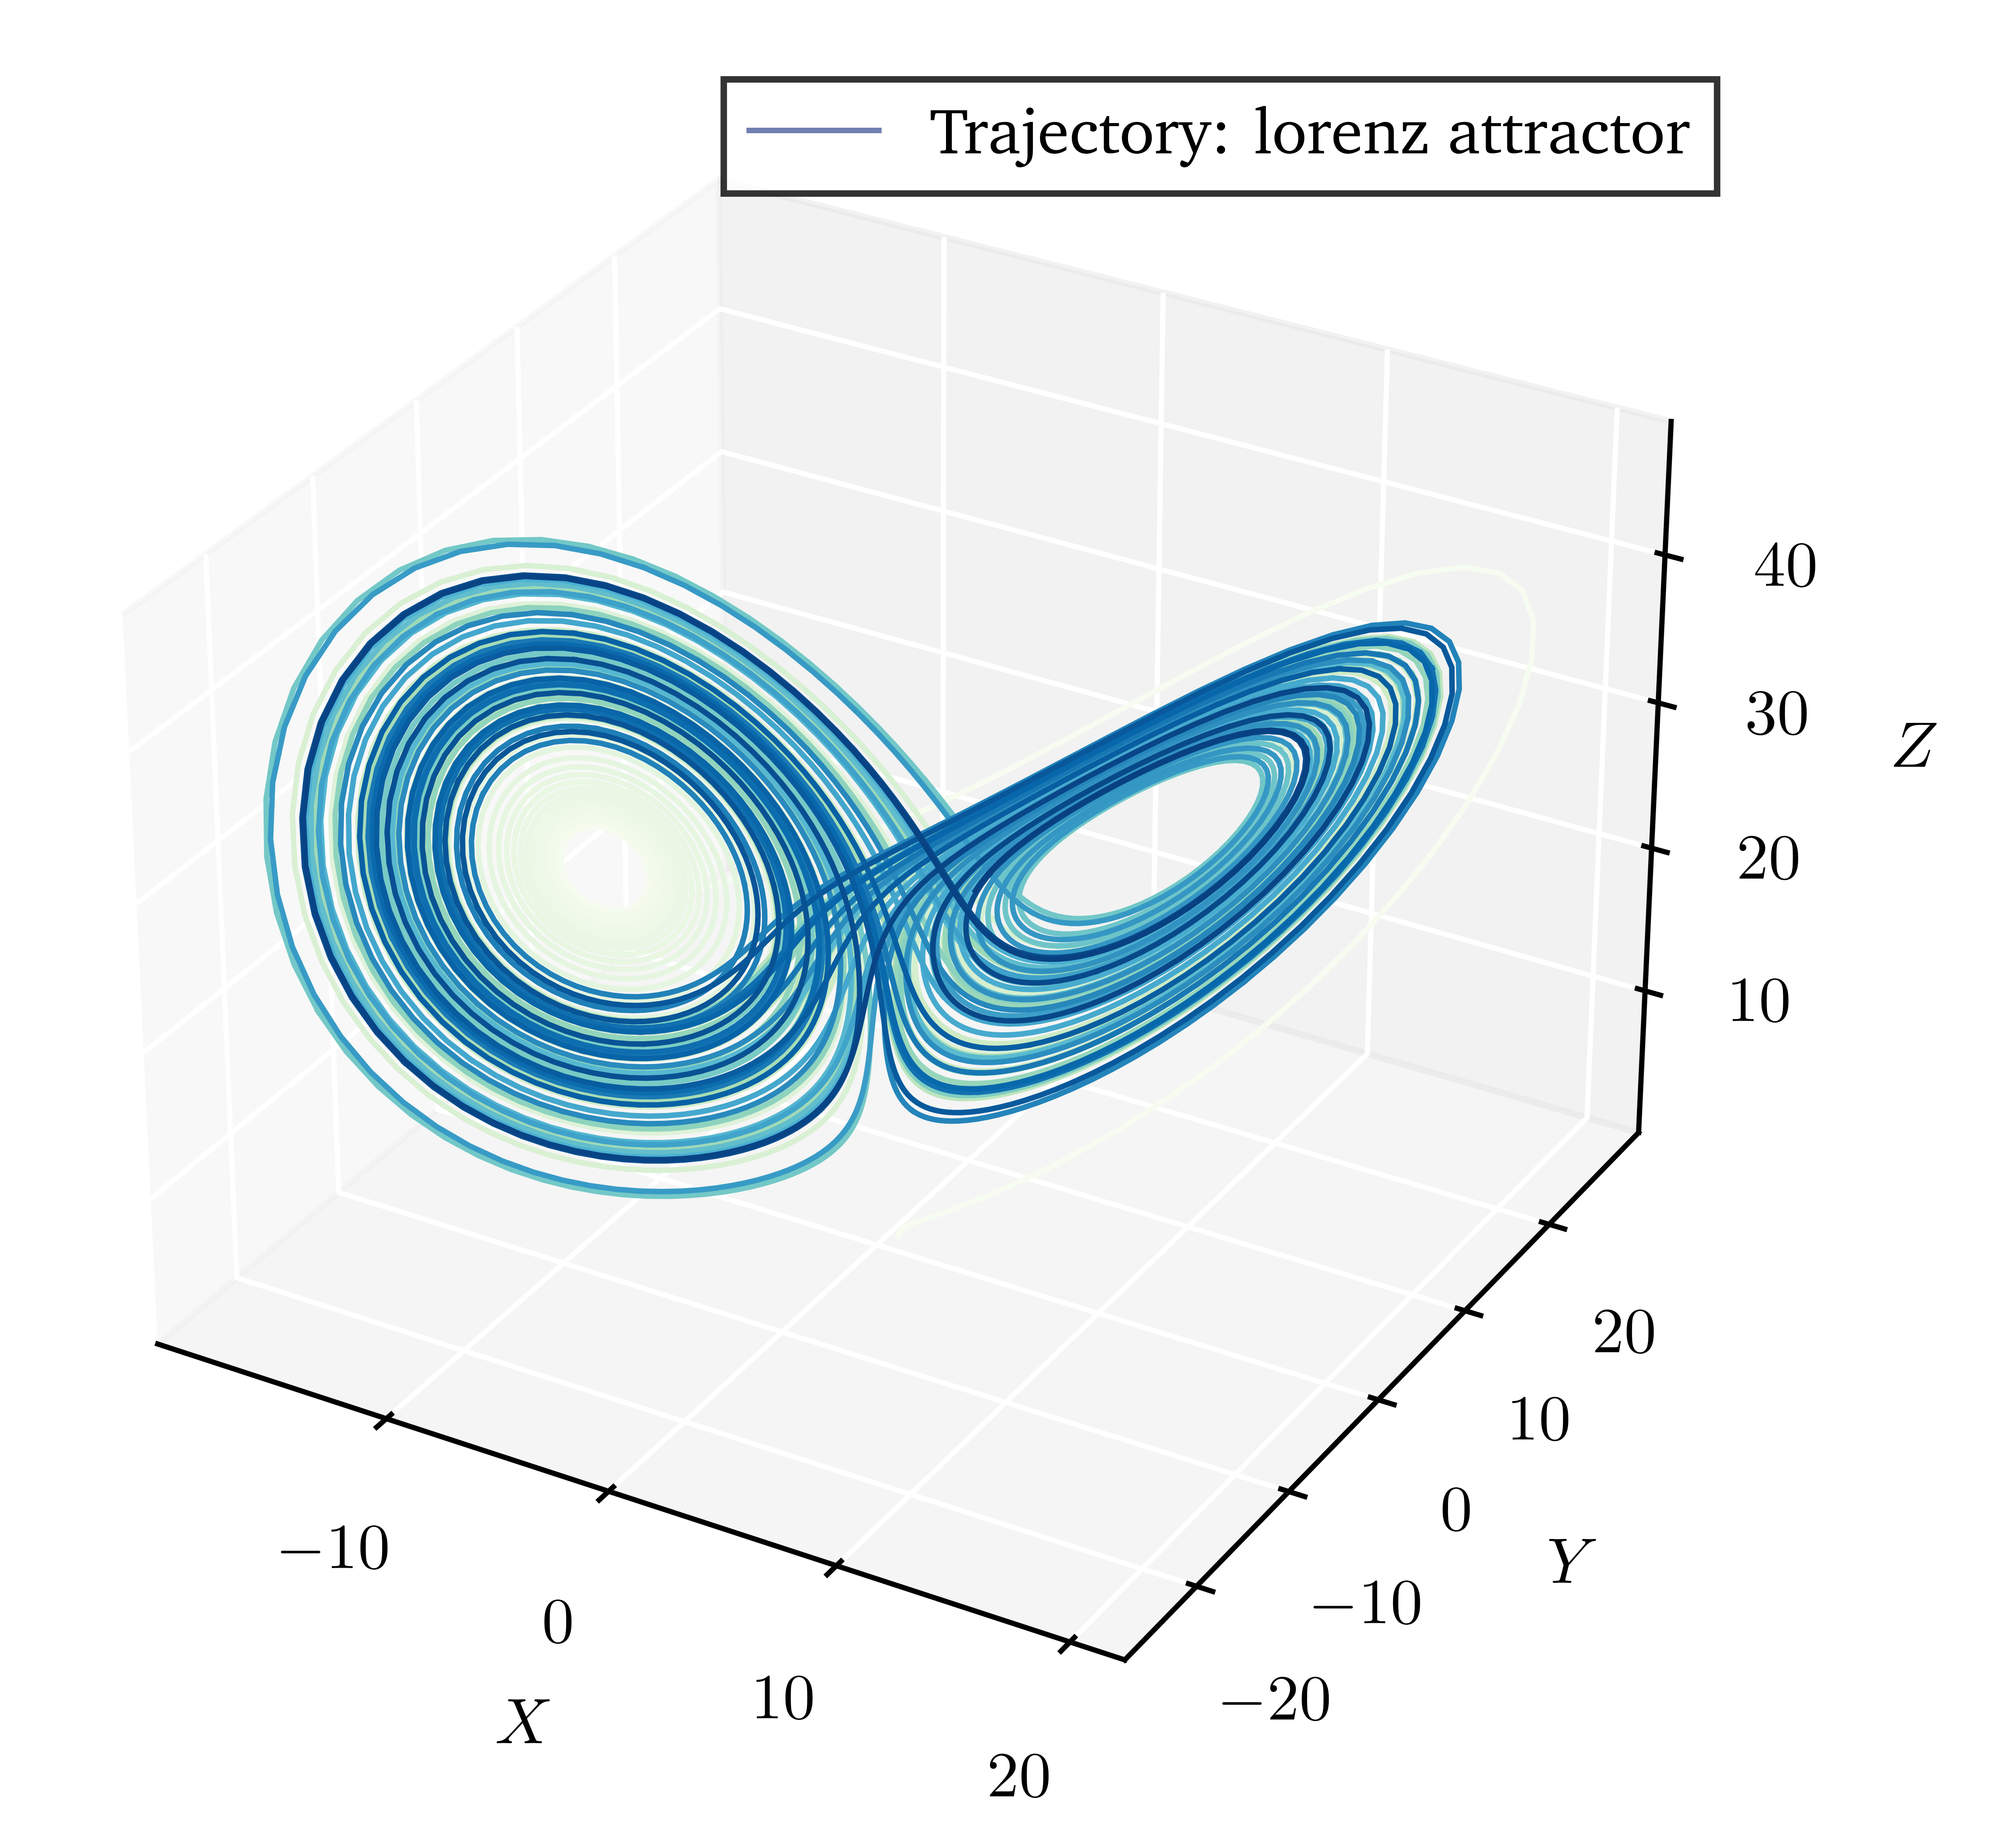
\includegraphics[scale=0.6]{figures/trajectories/traj_lorenz.png}
        \column{0.45\linewidth}
        \begin{itemize}
            \setlength\itemsep{1em}
            \item[$\diamond$] Conditions initiales $\bm{r} = (1, 0, -1)$ \\
            \item[$\diamond$] Temps de $100$ secondes
            \item[$\diamond$] Pas de $h = 0.01$
        \end{itemize}
    \end{columns}
\end{frame}

\begin{frame}
    \frametitle{Résultats - Trajectoires}
    \framesubtitle{Attracteur de Lorenz}
    \begin{columns}
        \column{0.5\linewidth}
        \centering
        \includegraphics[scale=0.55]{figures/trajectories/unicity_lorenz.png}
        \column{0.4\linewidth}
        Vérification qualitative du théorème d'unicité des solutions aux équations différentielles.
    \end{columns}
\end{frame}

\begin{frame}
    \frametitle{Résultats - Trajectoires}
    \framesubtitle{Attracteur de Rössler}
    \begin{columns}
        \column{0.55\linewidth}
        \centering
        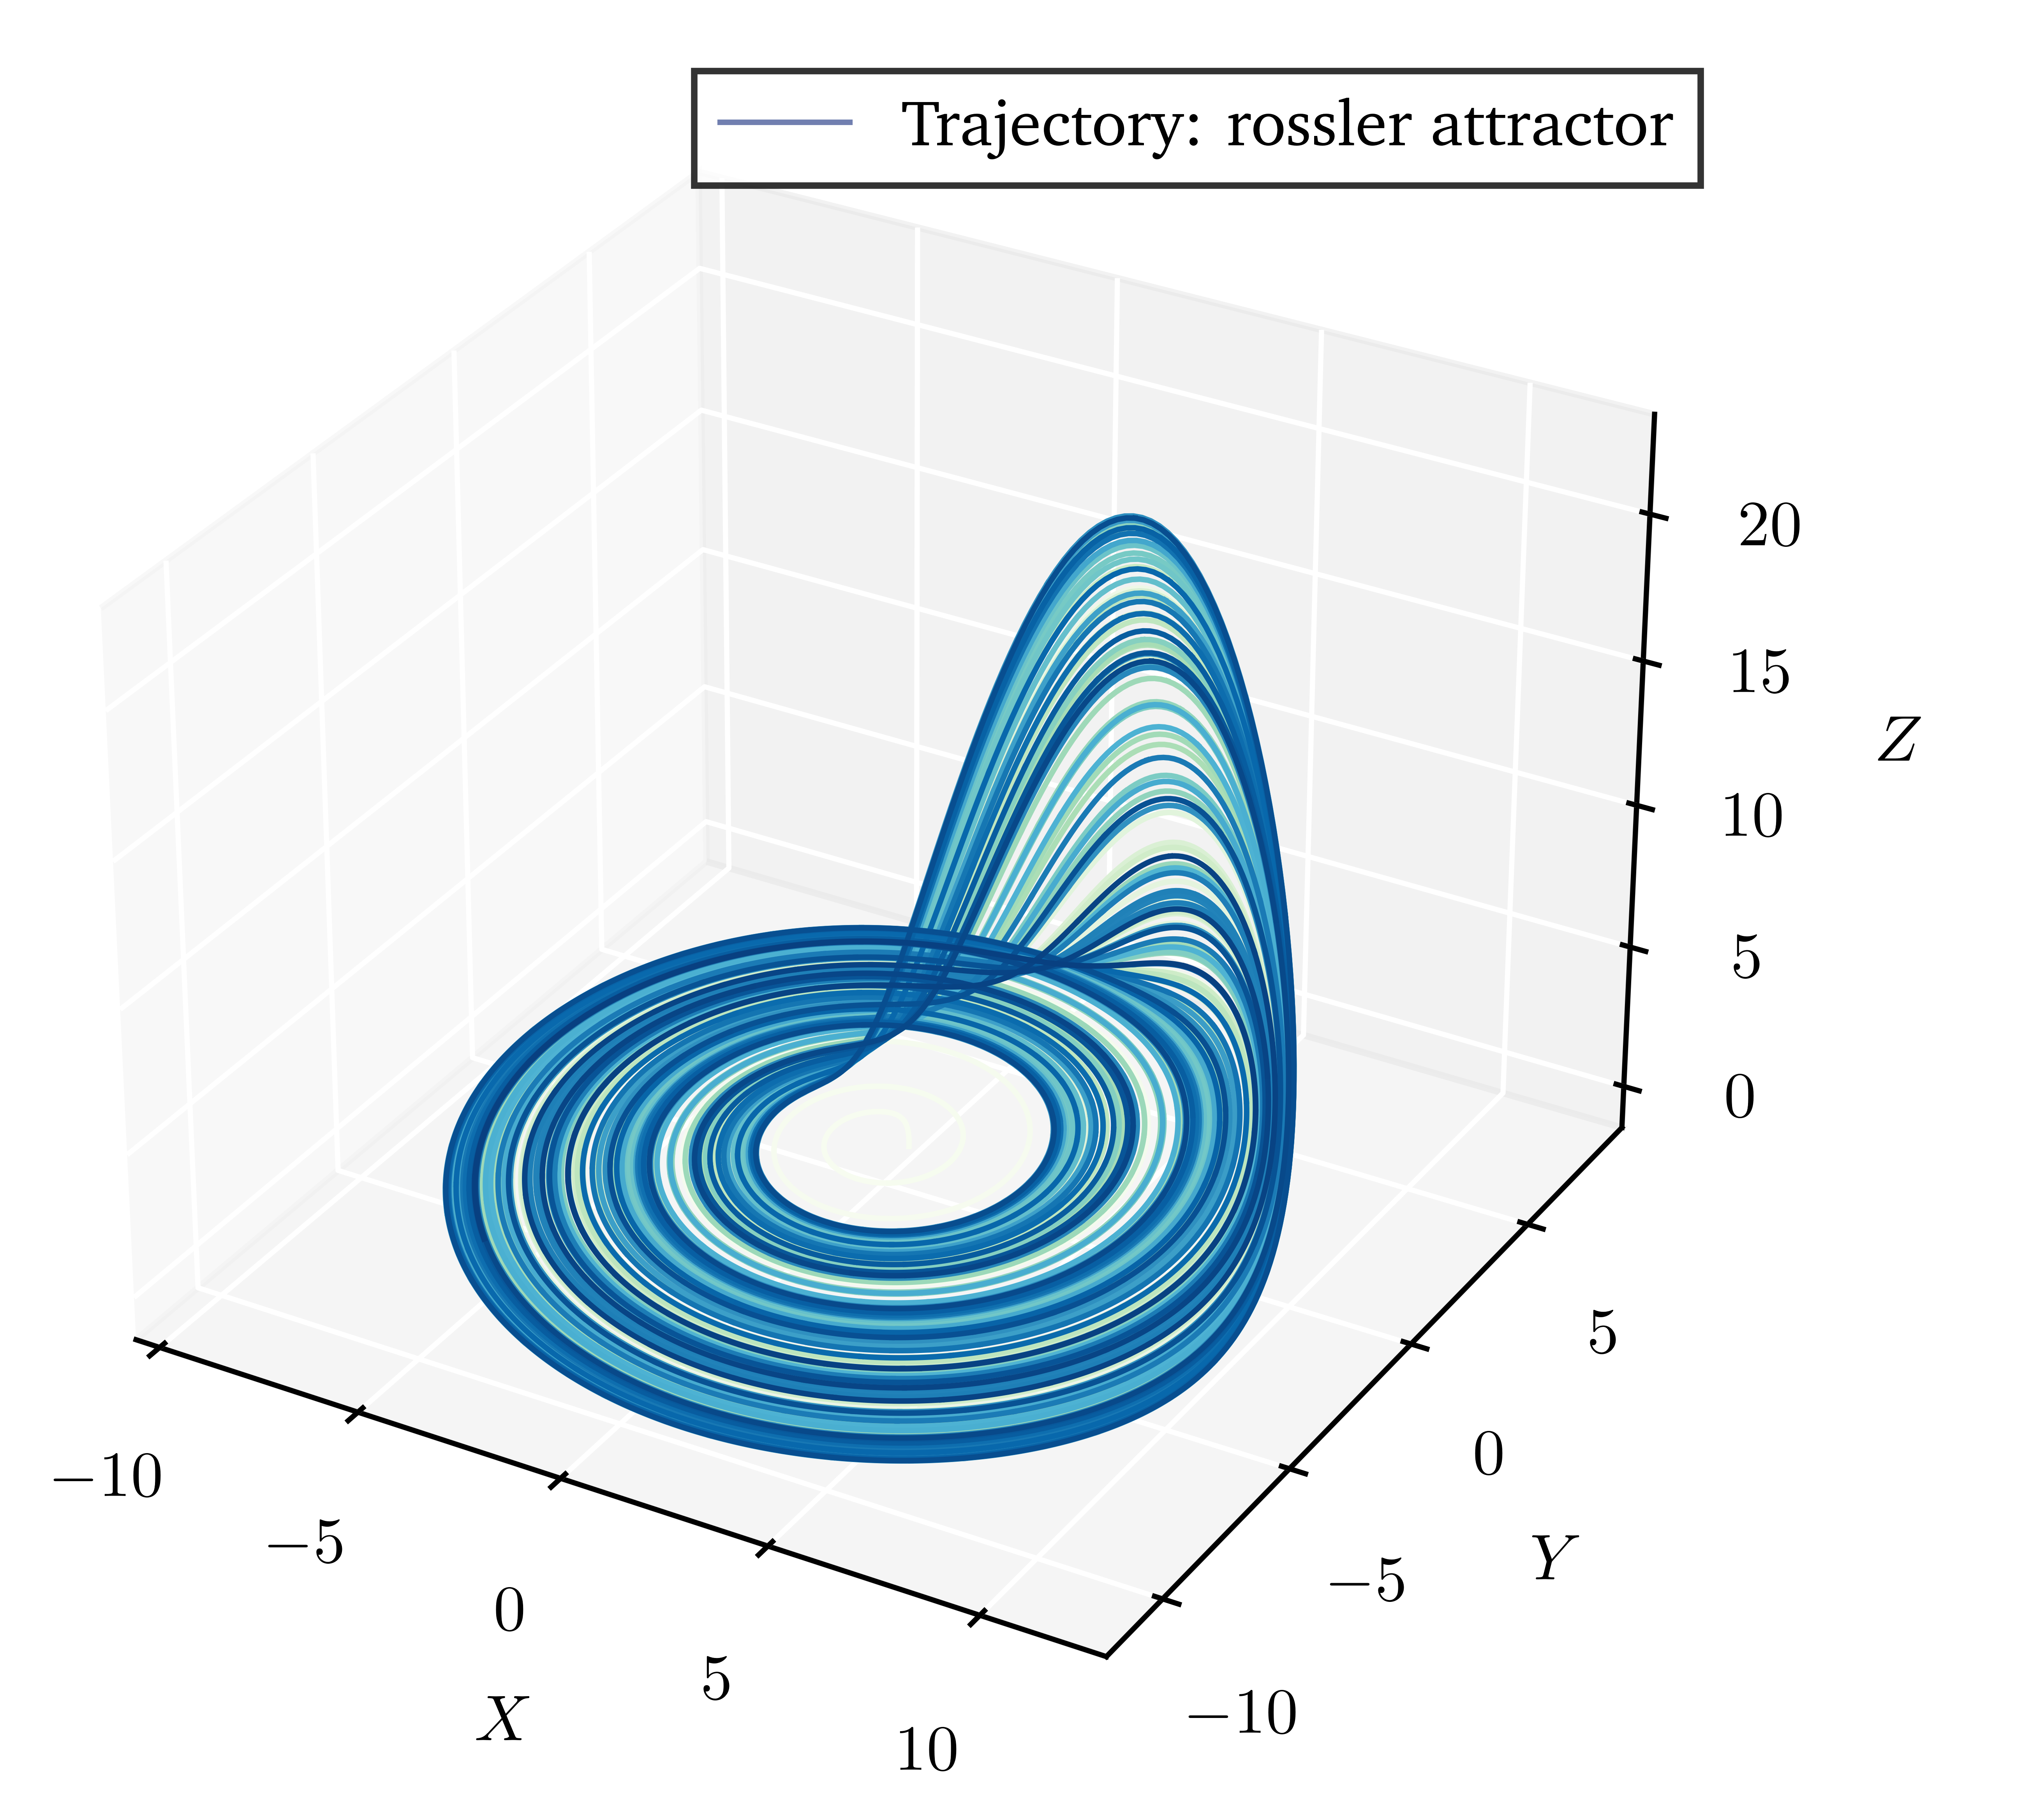
\includegraphics[scale=0.6]{figures/trajectories/traj_rossler.png}
        \column{0.45\linewidth}
        \begin{itemize}
            \setlength\itemsep{1em}
            \item[$\diamond$] Conditions initiales $\bm{r} = (1, 1, -1)$ \\
            \item[$\diamond$] Temps de $1000$ secondes
            \item[$\diamond$] Pas de $h = 0.001$
        \end{itemize}
    \end{columns}
\end{frame}

\begin{frame}
    \frametitle{Résultats - Trajectoires}
    \framesubtitle{Attracteur de Bouali}
    \begin{columns}
        \column{0.55\linewidth}
        \centering
        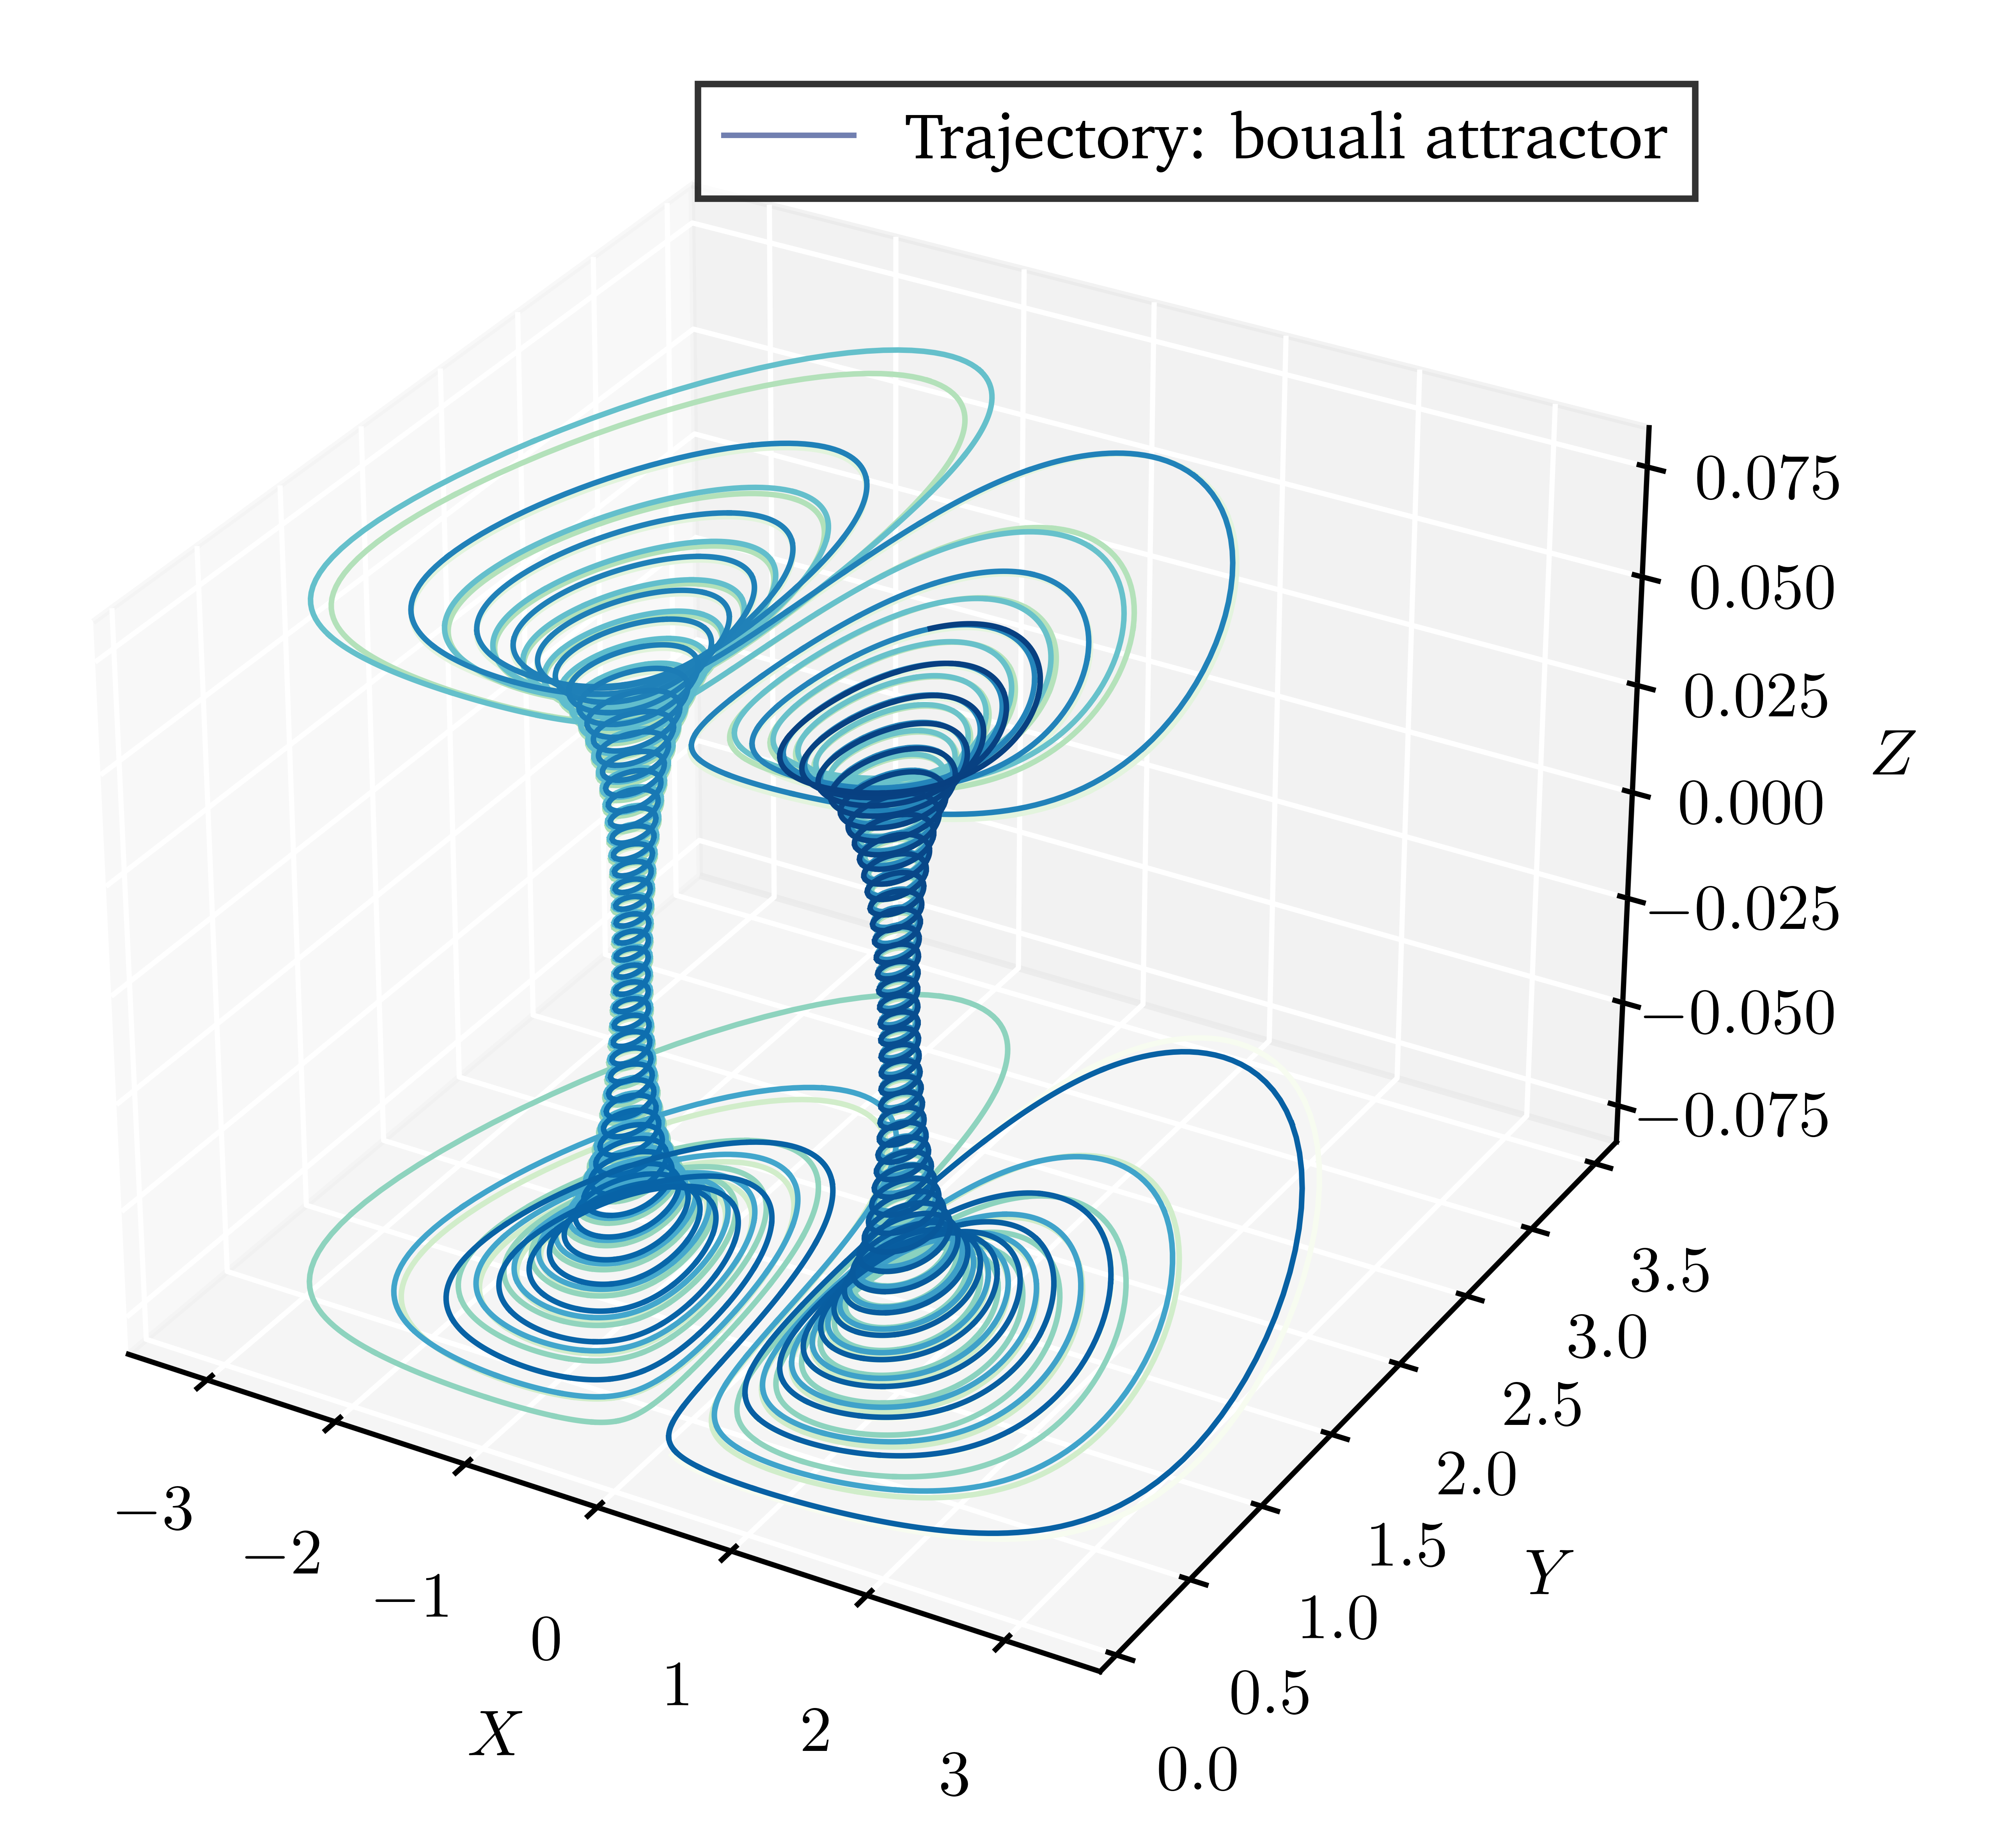
\includegraphics[scale=0.6]{figures/trajectories/traj_bouali.png}
        \column{0.45\linewidth}
        \begin{itemize}
            \setlength\itemsep{1em}
            \item[$\diamond$] Conditions initiales $\bm{r} = (0.2, 0.2, -0.08)$ \\
            \item[$\diamond$] Temps de $1000$ secondes
            \item[$\diamond$] Pas de $h = 0.001$
        \end{itemize}
    \end{columns}
\end{frame}

\begin{frame}
    \begin{center}
    \vspace{0.5cm}
    \boxed{
        Théorie - Spectre de Lyapunov \& Convergence
        }
    \end{center}
\end{frame}

\begin{frame}
    \frametitle{Théorie - Spectre de Lyapunov \& Convergence}
    \begin{columns}
        \column{0.55\linewidth}
        \centering
        \begin{figure}
            \begin{center}
                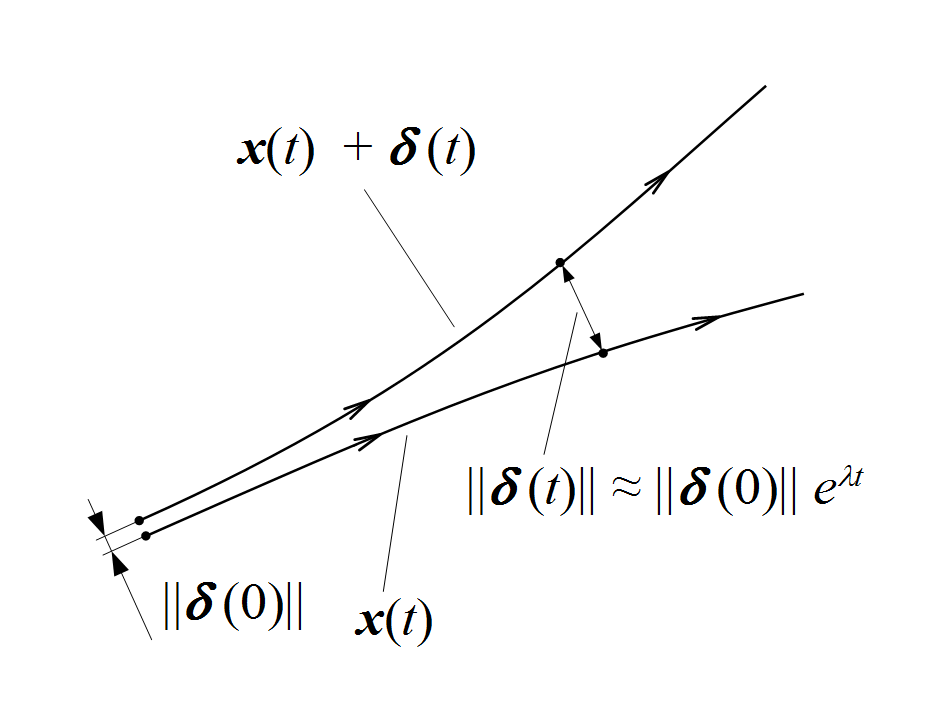
\includegraphics[scale=0.3]{figures/lyapunov_exponent.png}
            \end{center}
            \caption{Exposant de Lyapunov\footcite{LEswiki}.}
        \end{figure}
        \column{0.45\linewidth}
        \begin{itemize}
            \setlength\itemsep{1em}
            \item[$\diamond$] Le spectre de Lyapunov est de nature vectorielle
            \item[$\diamond$] Système dynamique de dimension $N$ $\implies\in\lambda_{i=1, 2\dots N}$ \\
        \end{itemize}
    \end{columns}
\end{frame}

\begin{frame}
    \frametitle{Théorie - Spectre de Lyapunov \& Convergence}
    Trois situations existent pour les exposants de Lyapunov $\lambda_j$:
    \vspace{0.5cm}
    \begin{itemize}
        \setlength\itemsep{1em}
        \item[$\diamond$] $\lambda_j > 0\implies$ signature chaotique
        \item[$\diamond$] $\lambda_j = 0\implies$ \textit{quasi-périodique}
        \item[$\diamond$] $\lambda_j < 0\implies$ convergence
    \end{itemize}
\end{frame}

\begin{frame}
    \frametitle{Théorie - Spectre de Lyapunov \& Convergence}
    L'équation qui permet d'obtenir l'exposant de Lyapunov dans la direction $j$ est
    \begin{align}
        \lambda_{j} = \lim_{n\to\infty}\frac{1}{n}\sum_{i = 0}^{n - 1}\ln(f^{(j)}(x_i))
    \end{align}
    \vspace{0.5cm}
    \begin{noteblock}{Note}
        Il est difficile de sommer un nombre infini numériquement. Quelles sont les solutions?
    \end{noteblock}
\end{frame}

\begin{frame}
    \begin{center}
    \vspace{0.5cm}
    \boxed{
        Méthodes numériques - Calculs matriciels \& Convergence
        }
    \end{center}
\end{frame}

\begin{frame}
    \frametitle{Méthodes numériques - Calculs matriciels \& Convergence}
    Numériquement, on procède de façon matricielle $\to$ $J$
    \vspace{0.5cm}
    \begin{defblock}{Définition: Matrice Jacobienne}
        Les éléments de la matrice jacobienne sont donnés par
        \begin{align}
            J_{ij} = \frac{\partial f_i}{\partial x_j},
        \end{align}
        où $f_i$ est l'équation $i$ et $x_j$ la variable de dérivation.
    \end{defblock}
\end{frame}

\begin{frame}
    \frametitle{Méthodes numériques - Calculs matriciels \& Convergence}
    Évolution volumique d'une sphère unitaire $U_{3x3}$ $\to$ taux de variation donnés par $J$. L'algorithme est qualitativement \pause
    \vspace{0.5cm}
    \begin{itemize}
        \setlength\itemsep{1em}
        \item[$\diamond$] Position sur la trajectoire $\bm{r}(t_n)$ \pause
        \item[$\diamond$] Évaluation de $J$ en ce point \pause
        \item[$\diamond$] Taux de contraction/expansion ($J\cdot U$) \pause
        \item[$\diamond$] Extraction du spectre de Lyapunov ($Q\cdot R$) \pause
        \item[$\diamond$] Mise à jours des perturbations de l'espace des phases au temps $t_n$
    \end{itemize}
\end{frame}

\begin{frame}
    \frametitle{Méthodes numériques - Calculs matriciels \& Convergence}
    \begin{columns}
        \column{0.5\linewidth}
        \centering
        \begin{figure}
            \begin{center}
                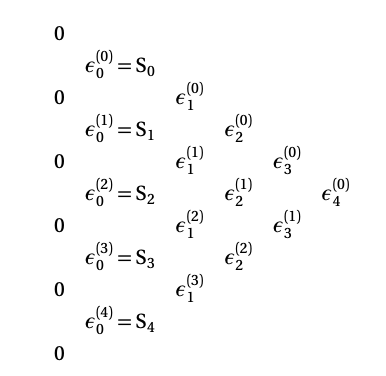
\includegraphics[scale=0.4]{figures/epsilon_tri_array.png}
            \end{center}
            \caption{\parencite{SENECH}.}
        \end{figure}
        \column{0.5\linewidth}
        Convergence du spectre de Lyapunov dans la limite $t\to\infty$ grâce à l'algorithme \textit{epsilon}
    \end{columns}
\end{frame}

\begin{frame}
    \begin{center}
    \vspace{0.5cm}
        \boxed{
        Résultats - Spectre de Lyapunov
        }
    \end{center}
\end{frame}

\begin{frame}
    \frametitle{Résultats - Spectre de Lyapunov}
    \framesubtitle{Attracteur de Lorenz}
    Simulation pour 100 secondes avec $10^4$ points et $\bm{r}_0 = (1, 0, -1)$
    \vspace{1cm}
    \begin{columns}
        \column{0.5\linewidth}
        \centering
        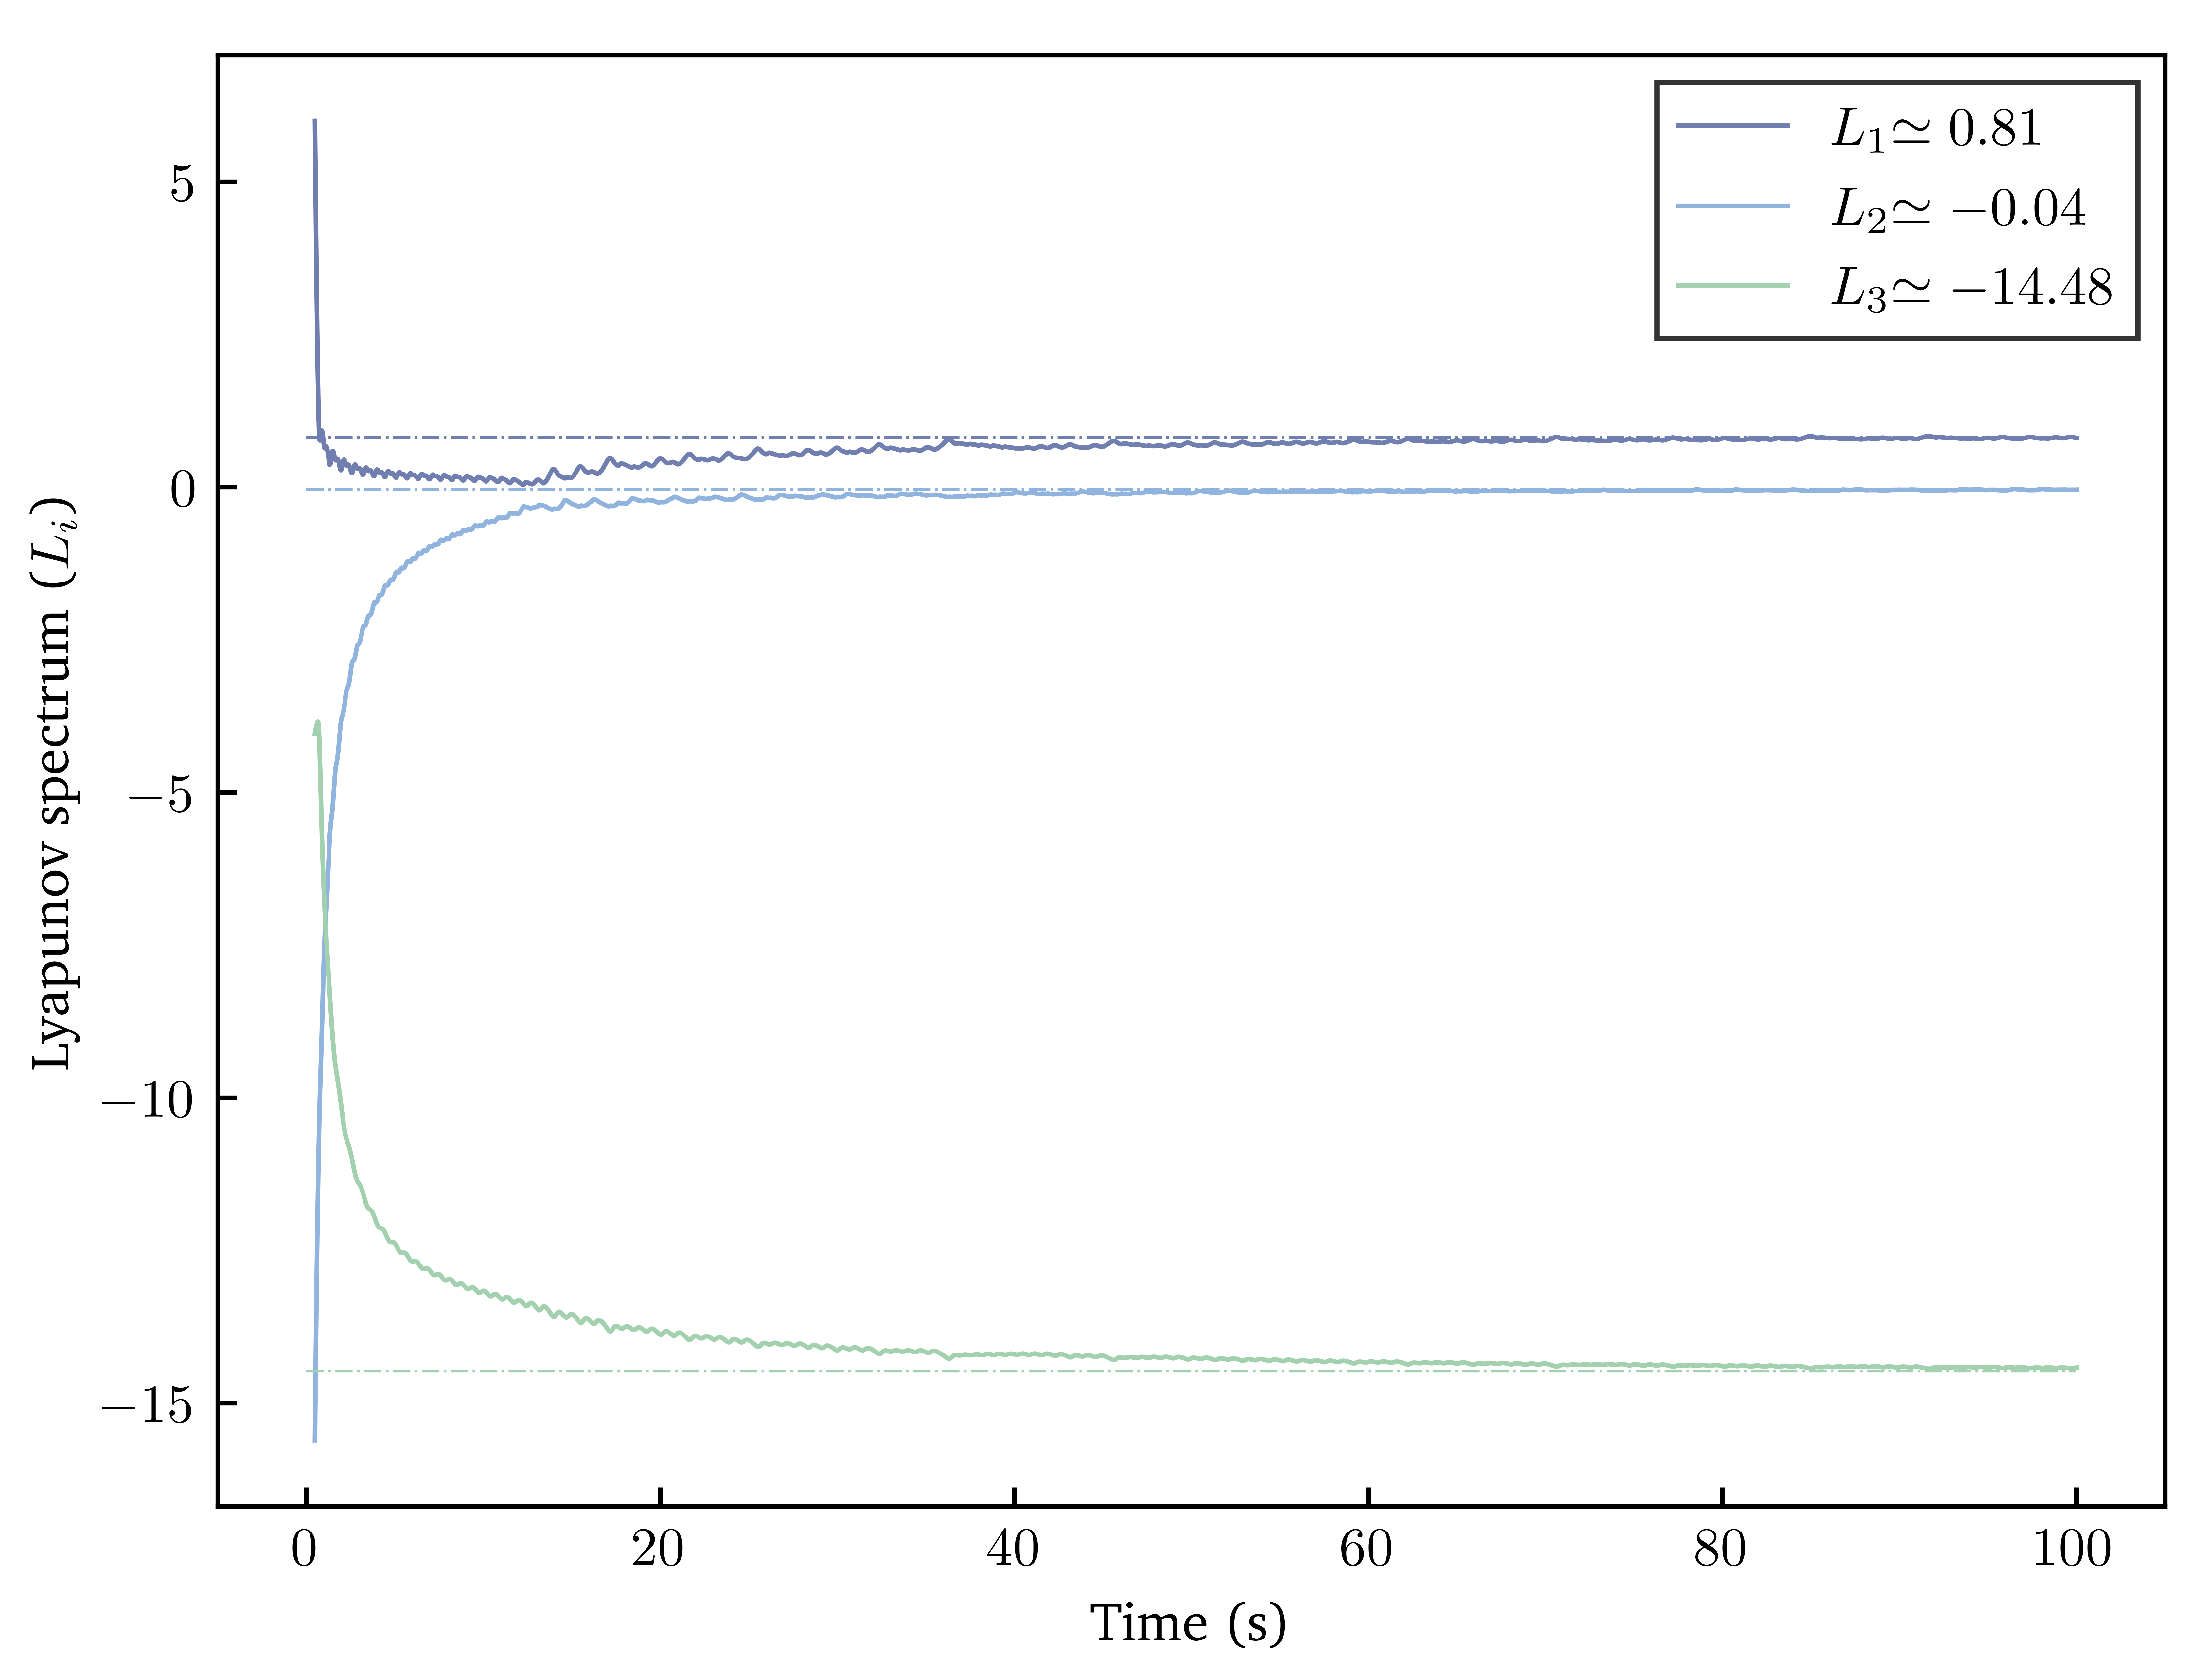
\includegraphics[scale=0.4]{figures/lyapunovs/lyap_lorenz.png}
        \column{0.5\linewidth}
        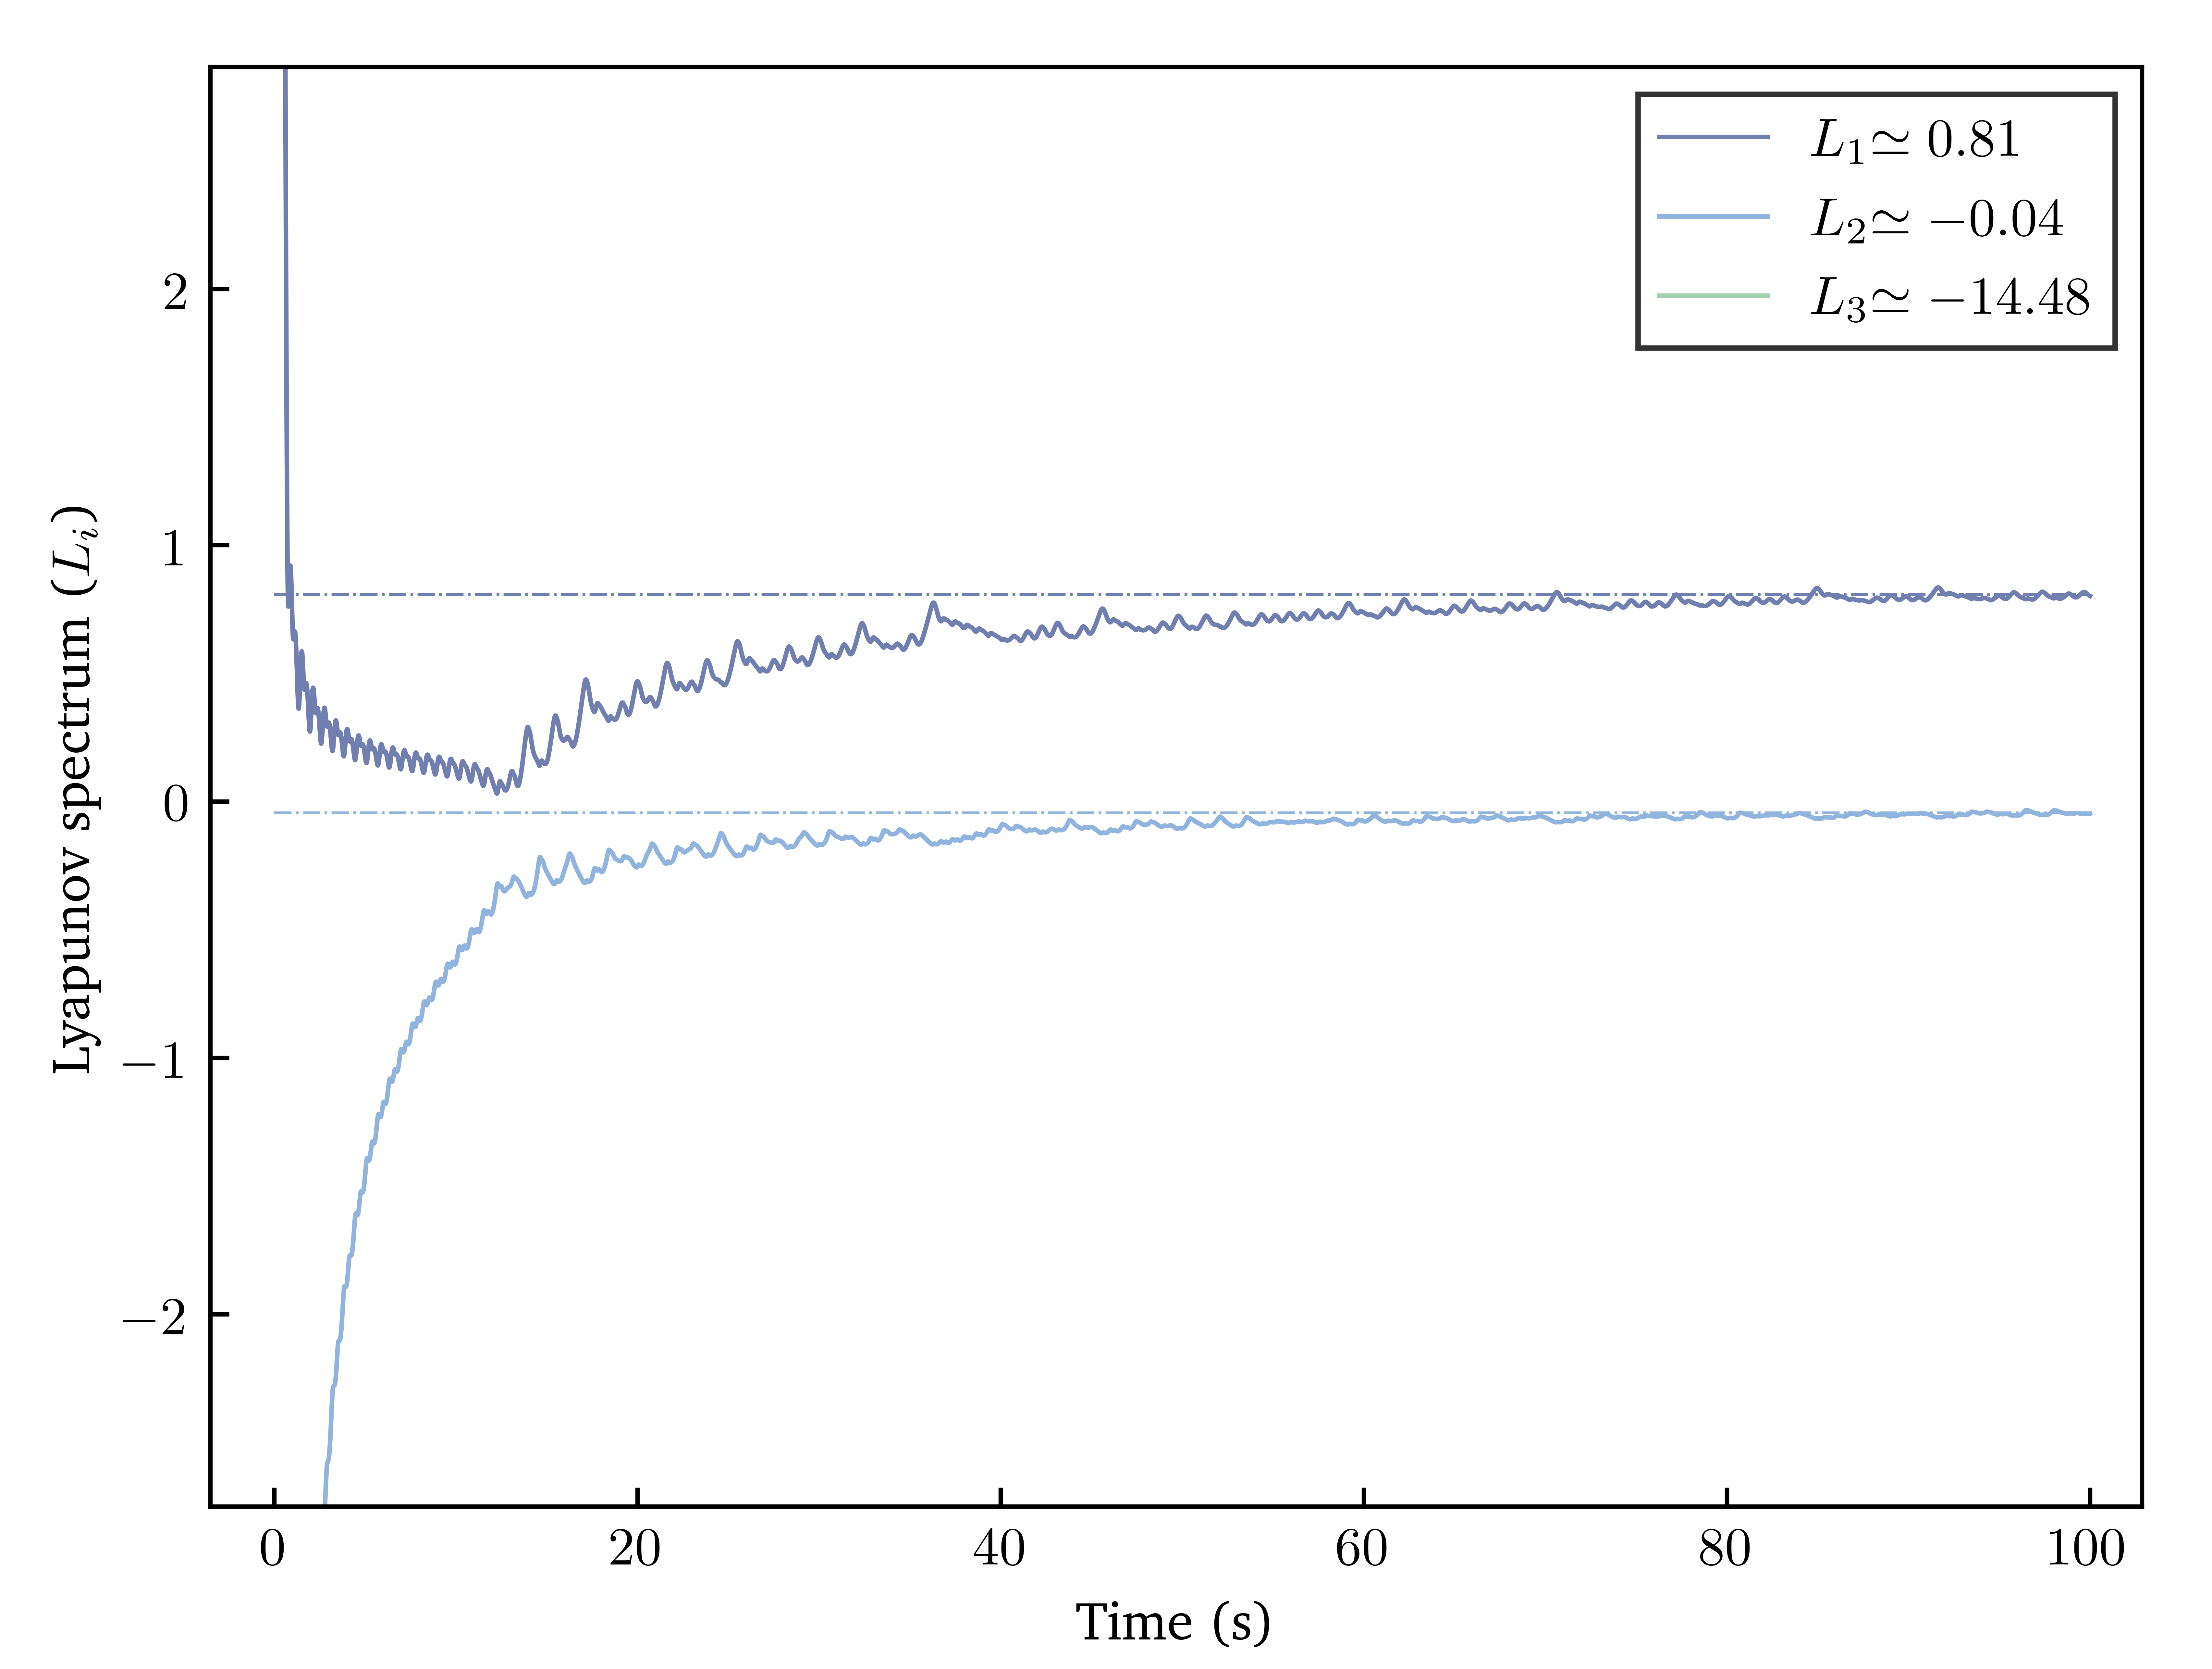
\includegraphics[scale=0.4]{figures/lyapunovs/lyap_lorenz_zoom.png}
    \end{columns}
\end{frame}

\begin{frame}
    \frametitle{Résultats - Spectre de Lyapunov}
    \framesubtitle{Attracteur de Rössler}
    Simulation pour 500 secondes avec $10^5$ points et $\bm{r}_0 = (1, 1, -1)$
    \vspace{1cm}
    \begin{columns}
        \column{0.5\linewidth}
        \centering
        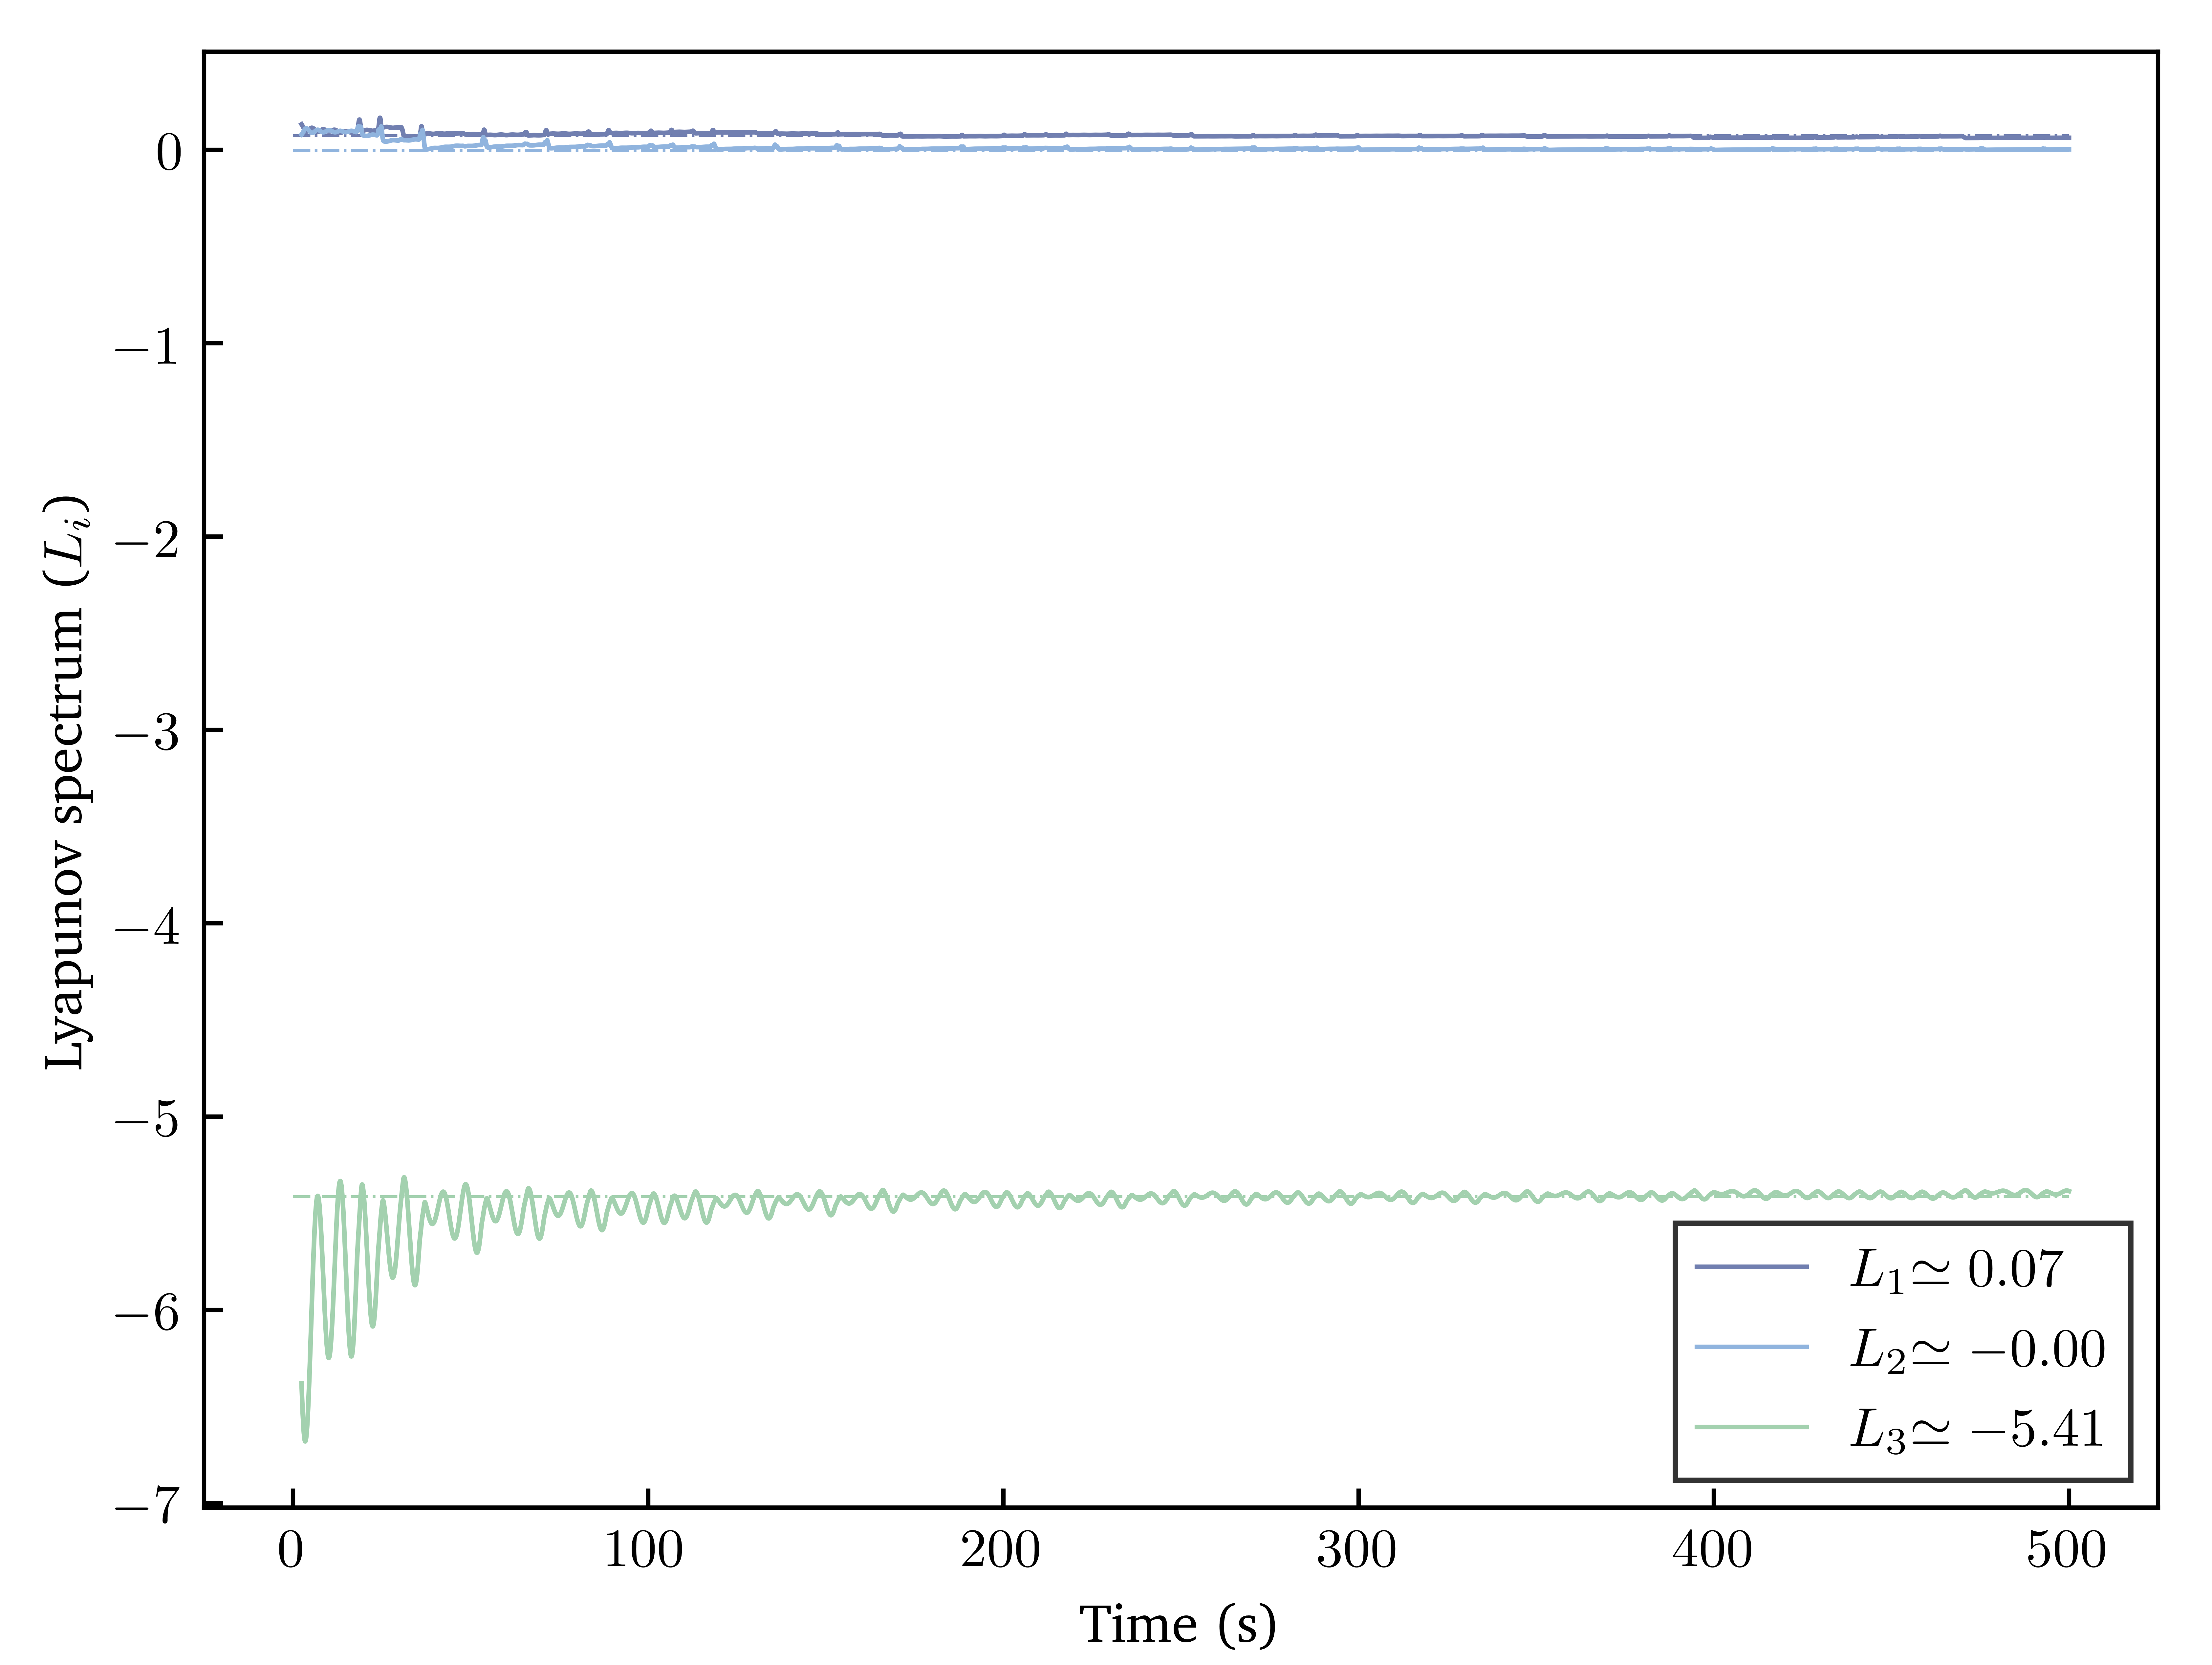
\includegraphics[scale=0.4]{figures/lyapunovs/lyap_rossler.png}
        \column{0.5\linewidth}
        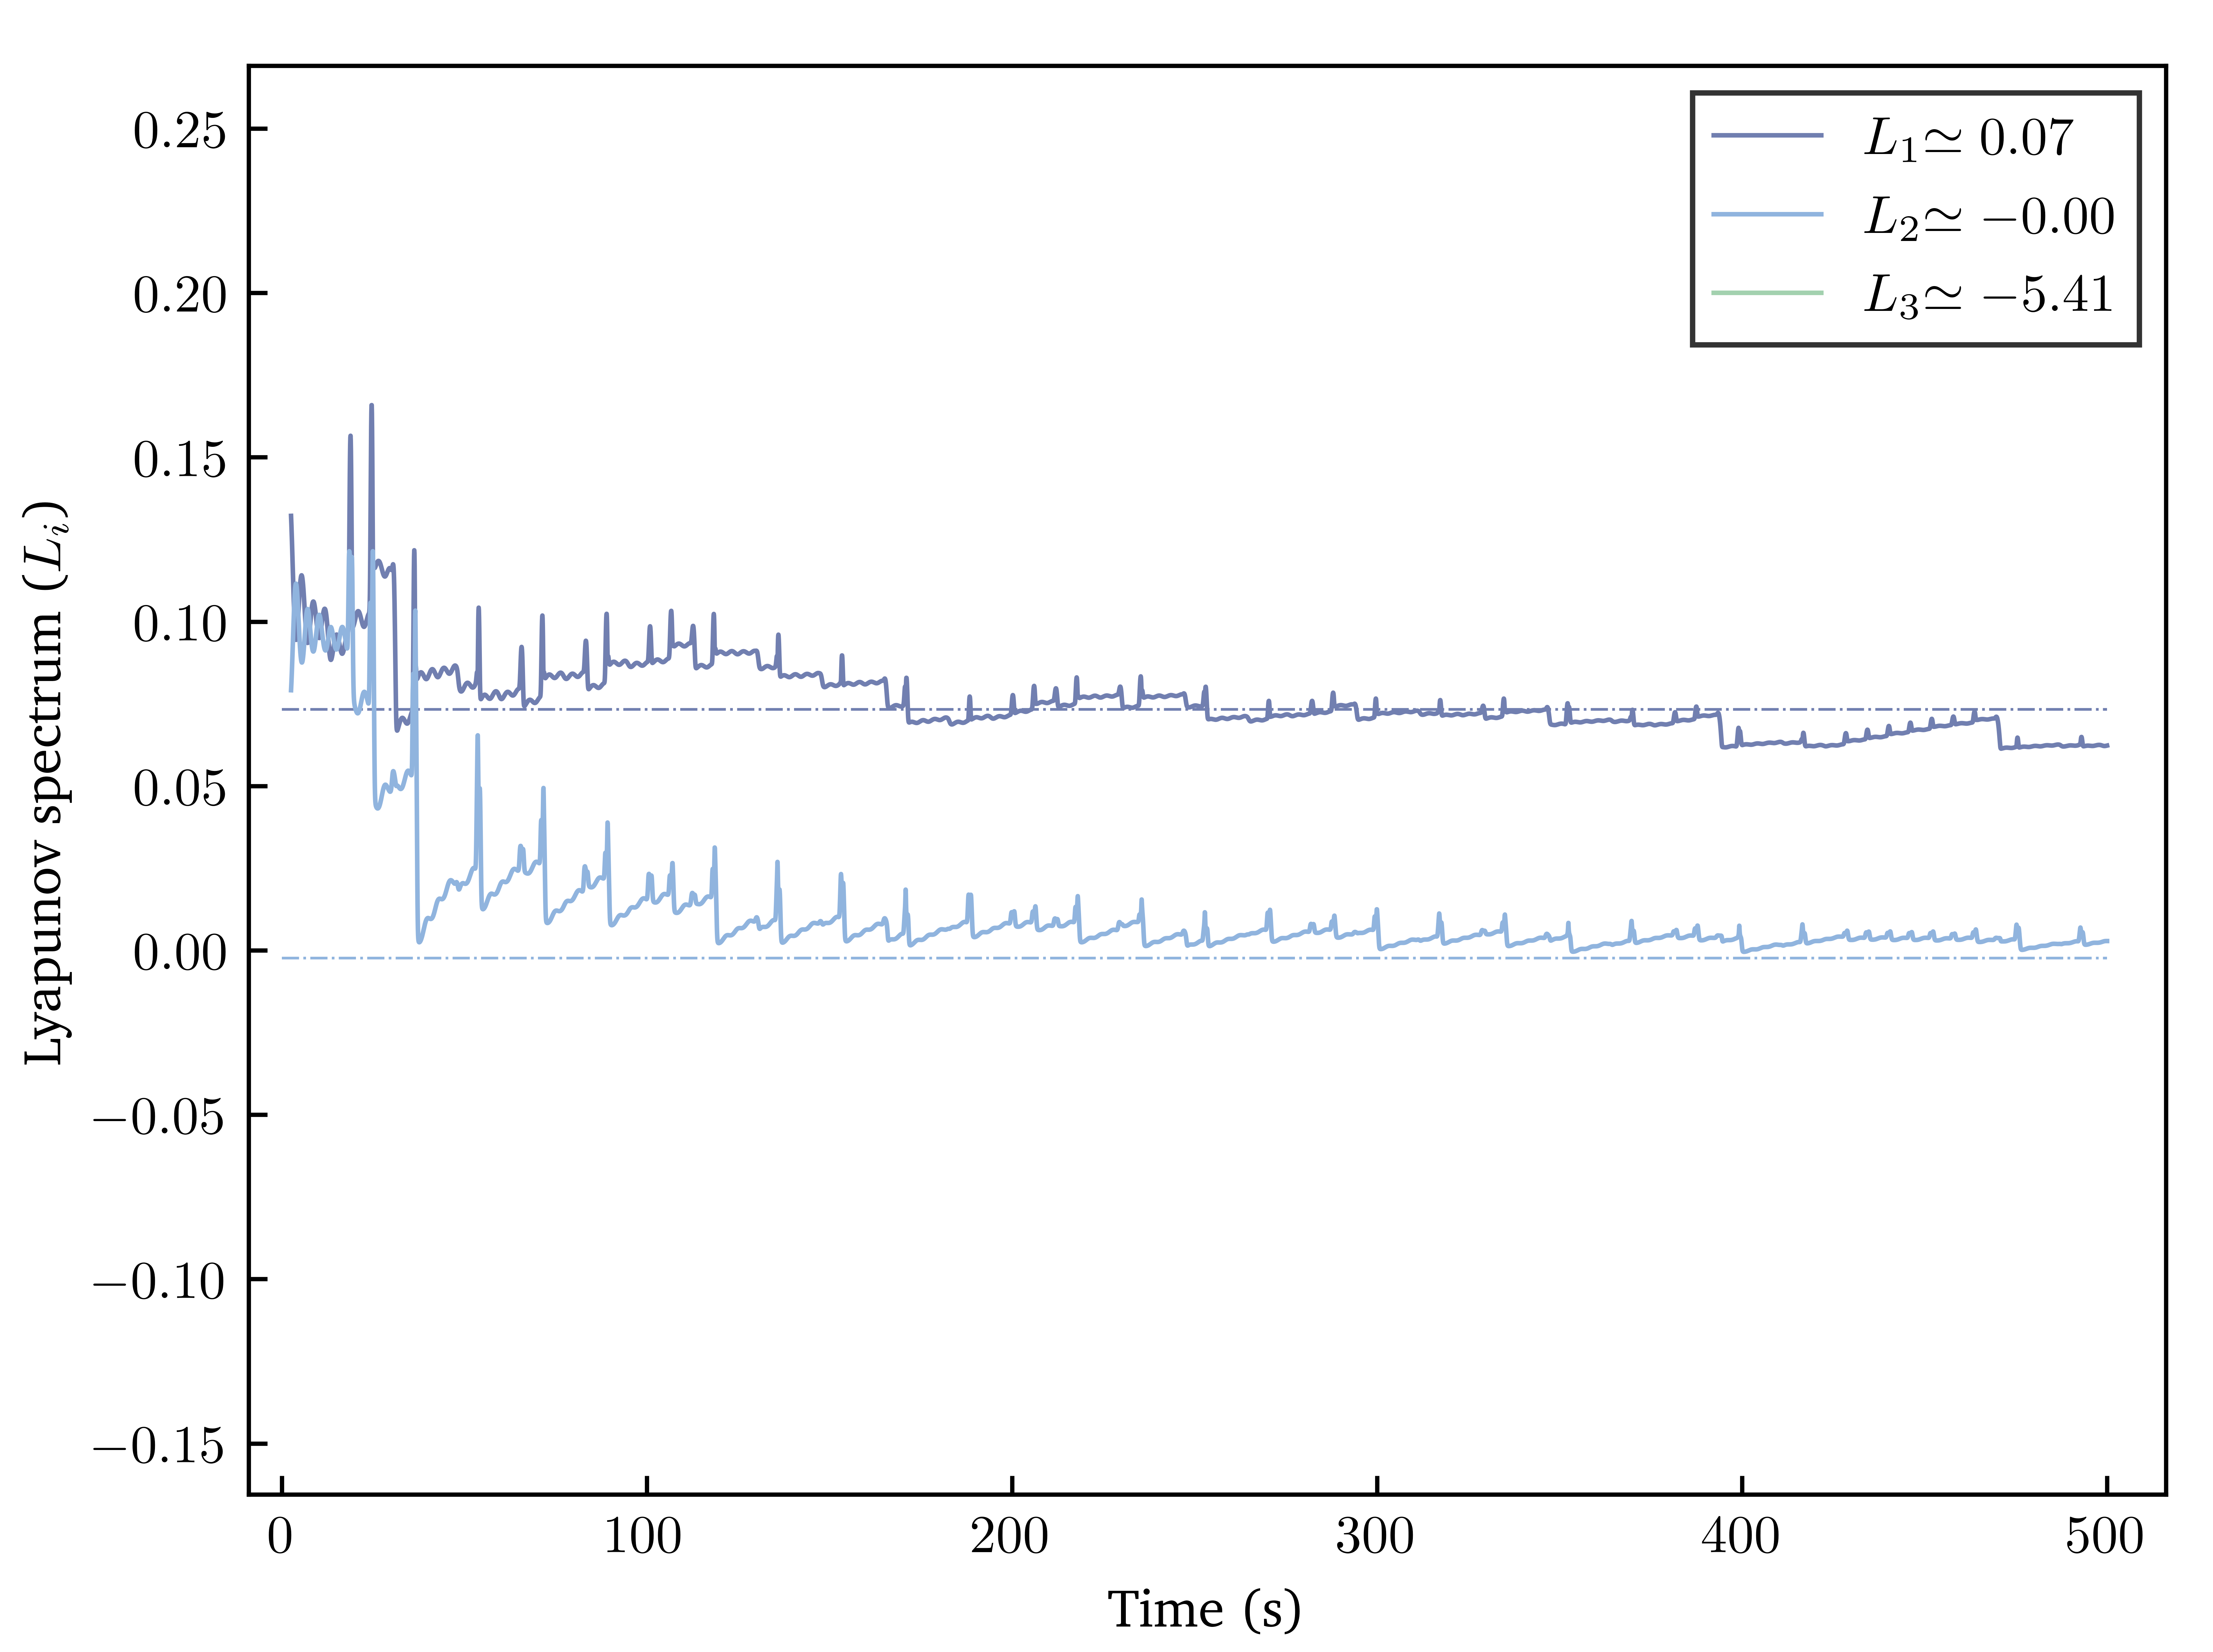
\includegraphics[scale=0.4]{figures/lyapunovs/lyap_rossler_zoom.png}
    \end{columns}
\end{frame}

\begin{frame}
    \frametitle{Résultats - Spectre de Lyapunov}
    \framesubtitle{Attracteur de Bouali}
    Simulation pour 500 secondes avec $10^5$ points et $\bm{r}_0 = (0.2, 0.2, -0.08)$
    \vspace{1cm}
    \begin{columns}
        \column{0.5\linewidth}
        \centering
        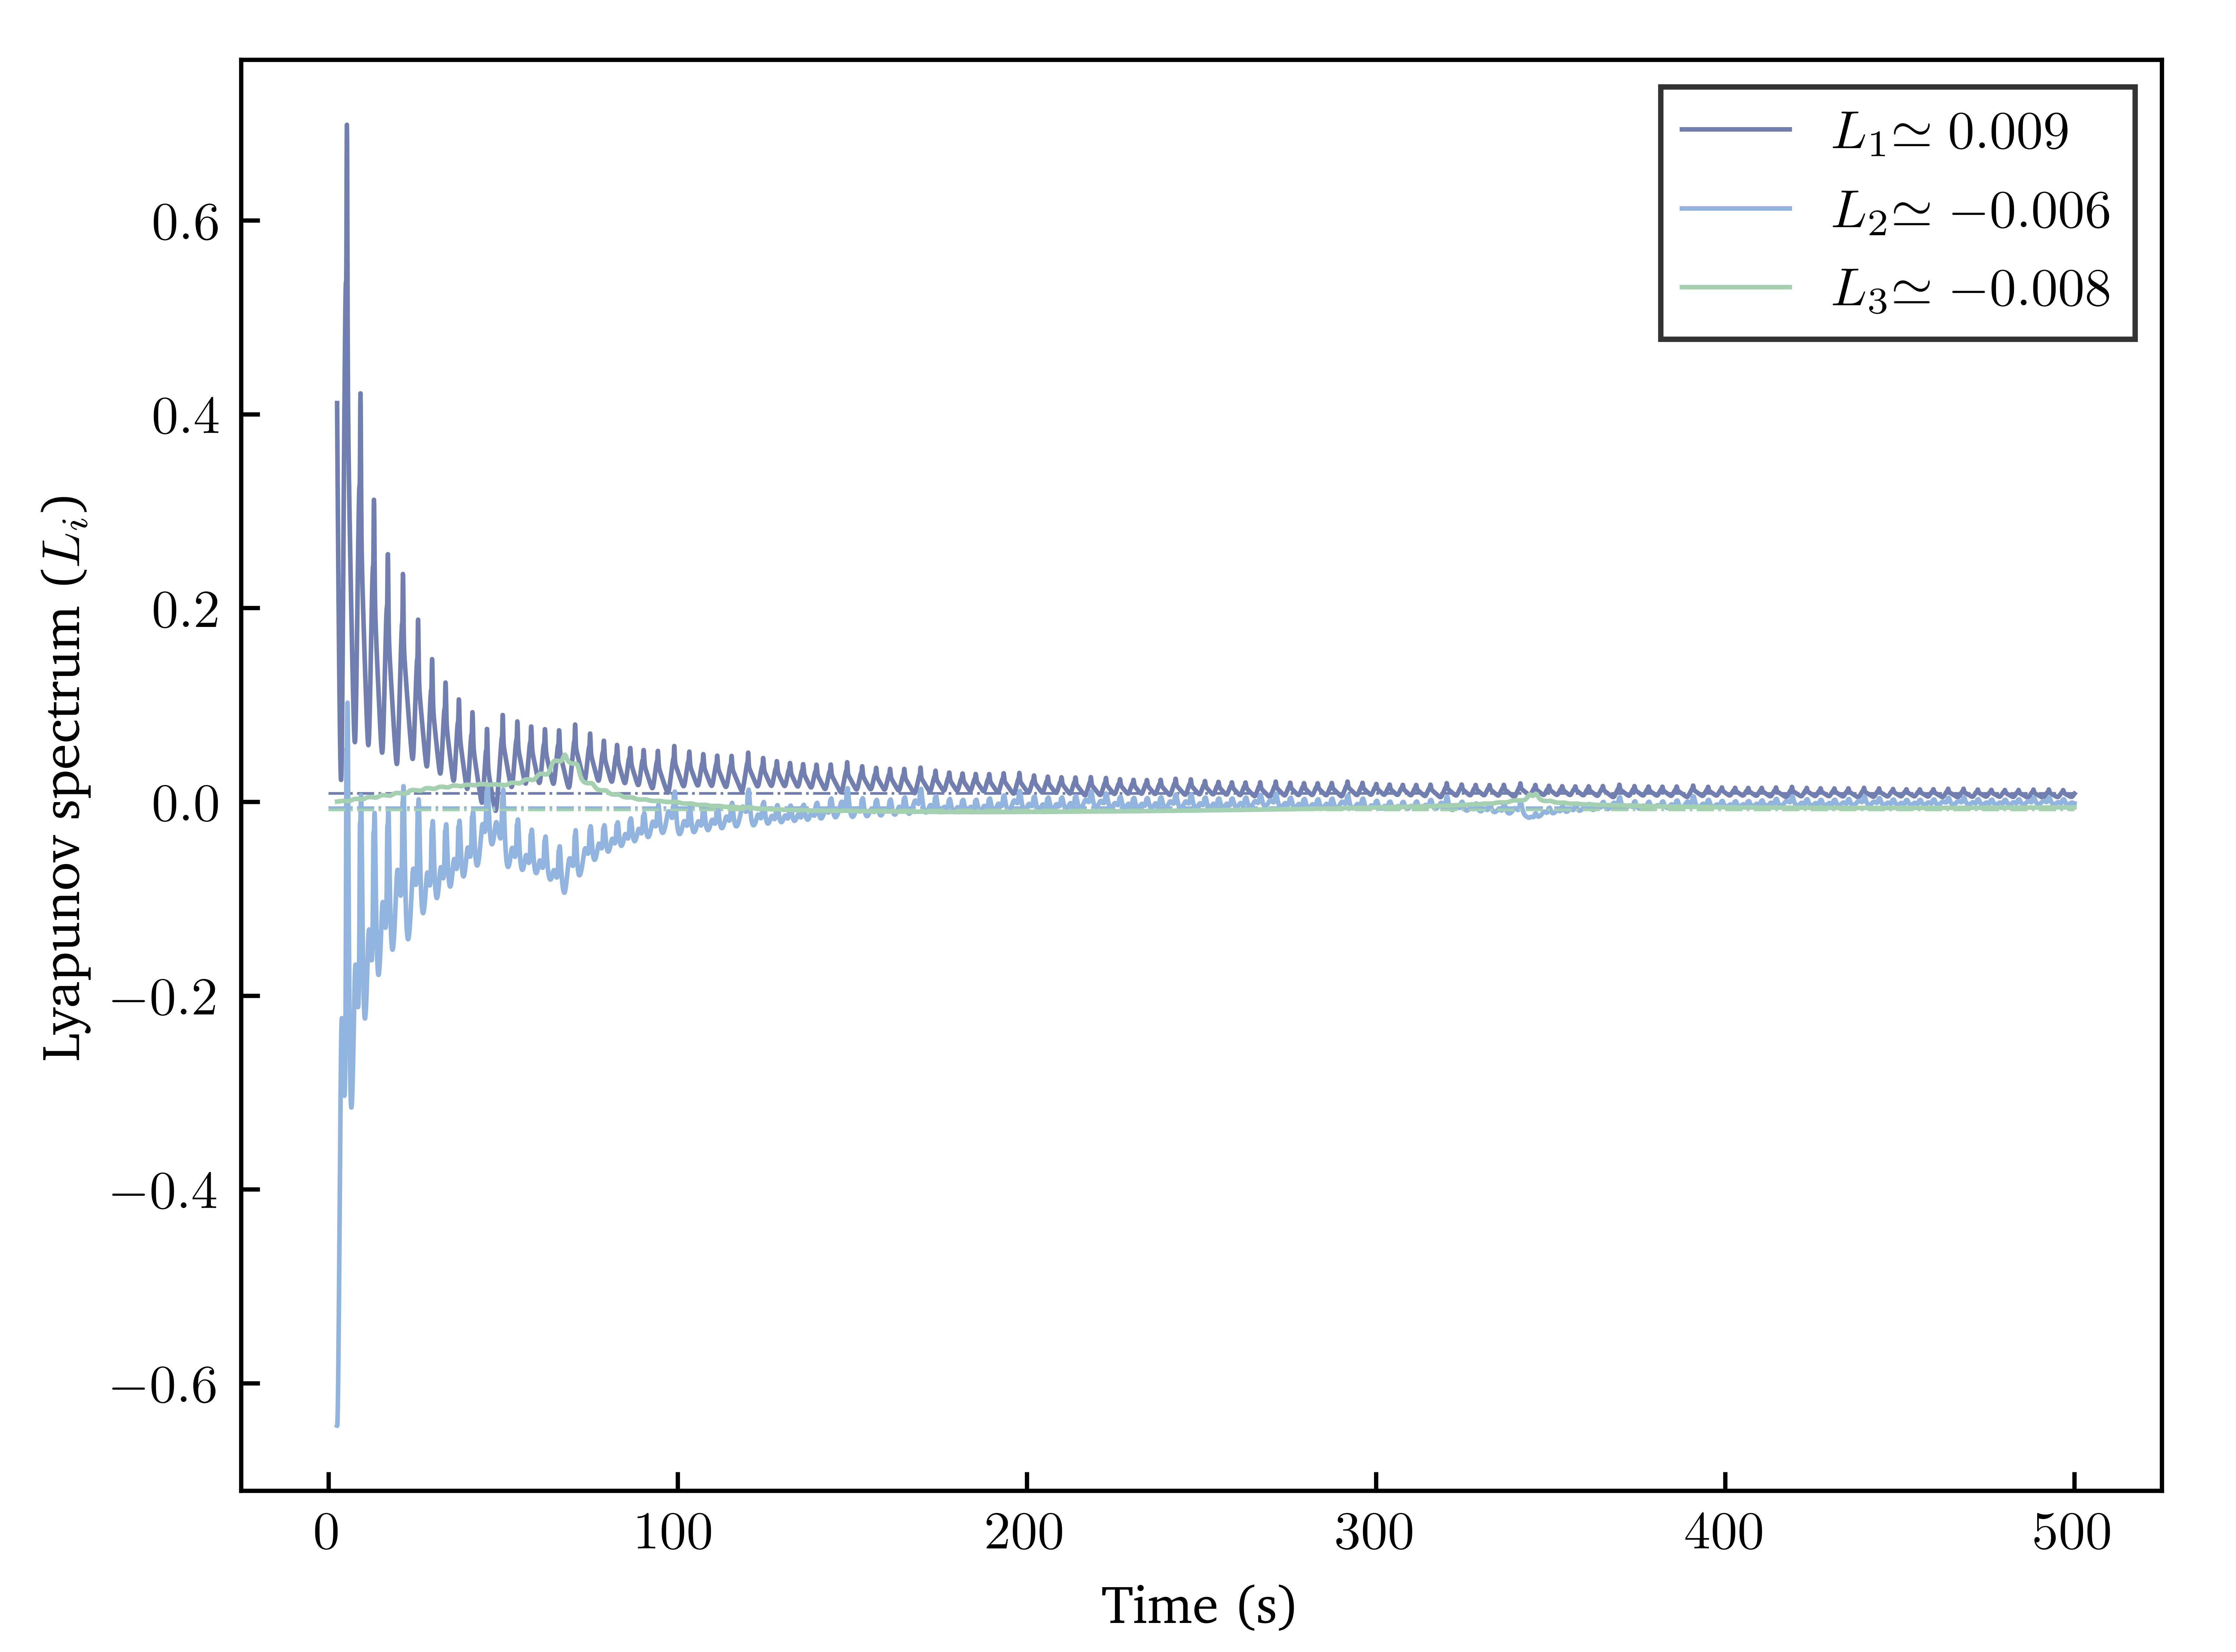
\includegraphics[scale=0.4]{figures/lyapunovs/lyap_bouali.png}
        \column{0.5\linewidth}
        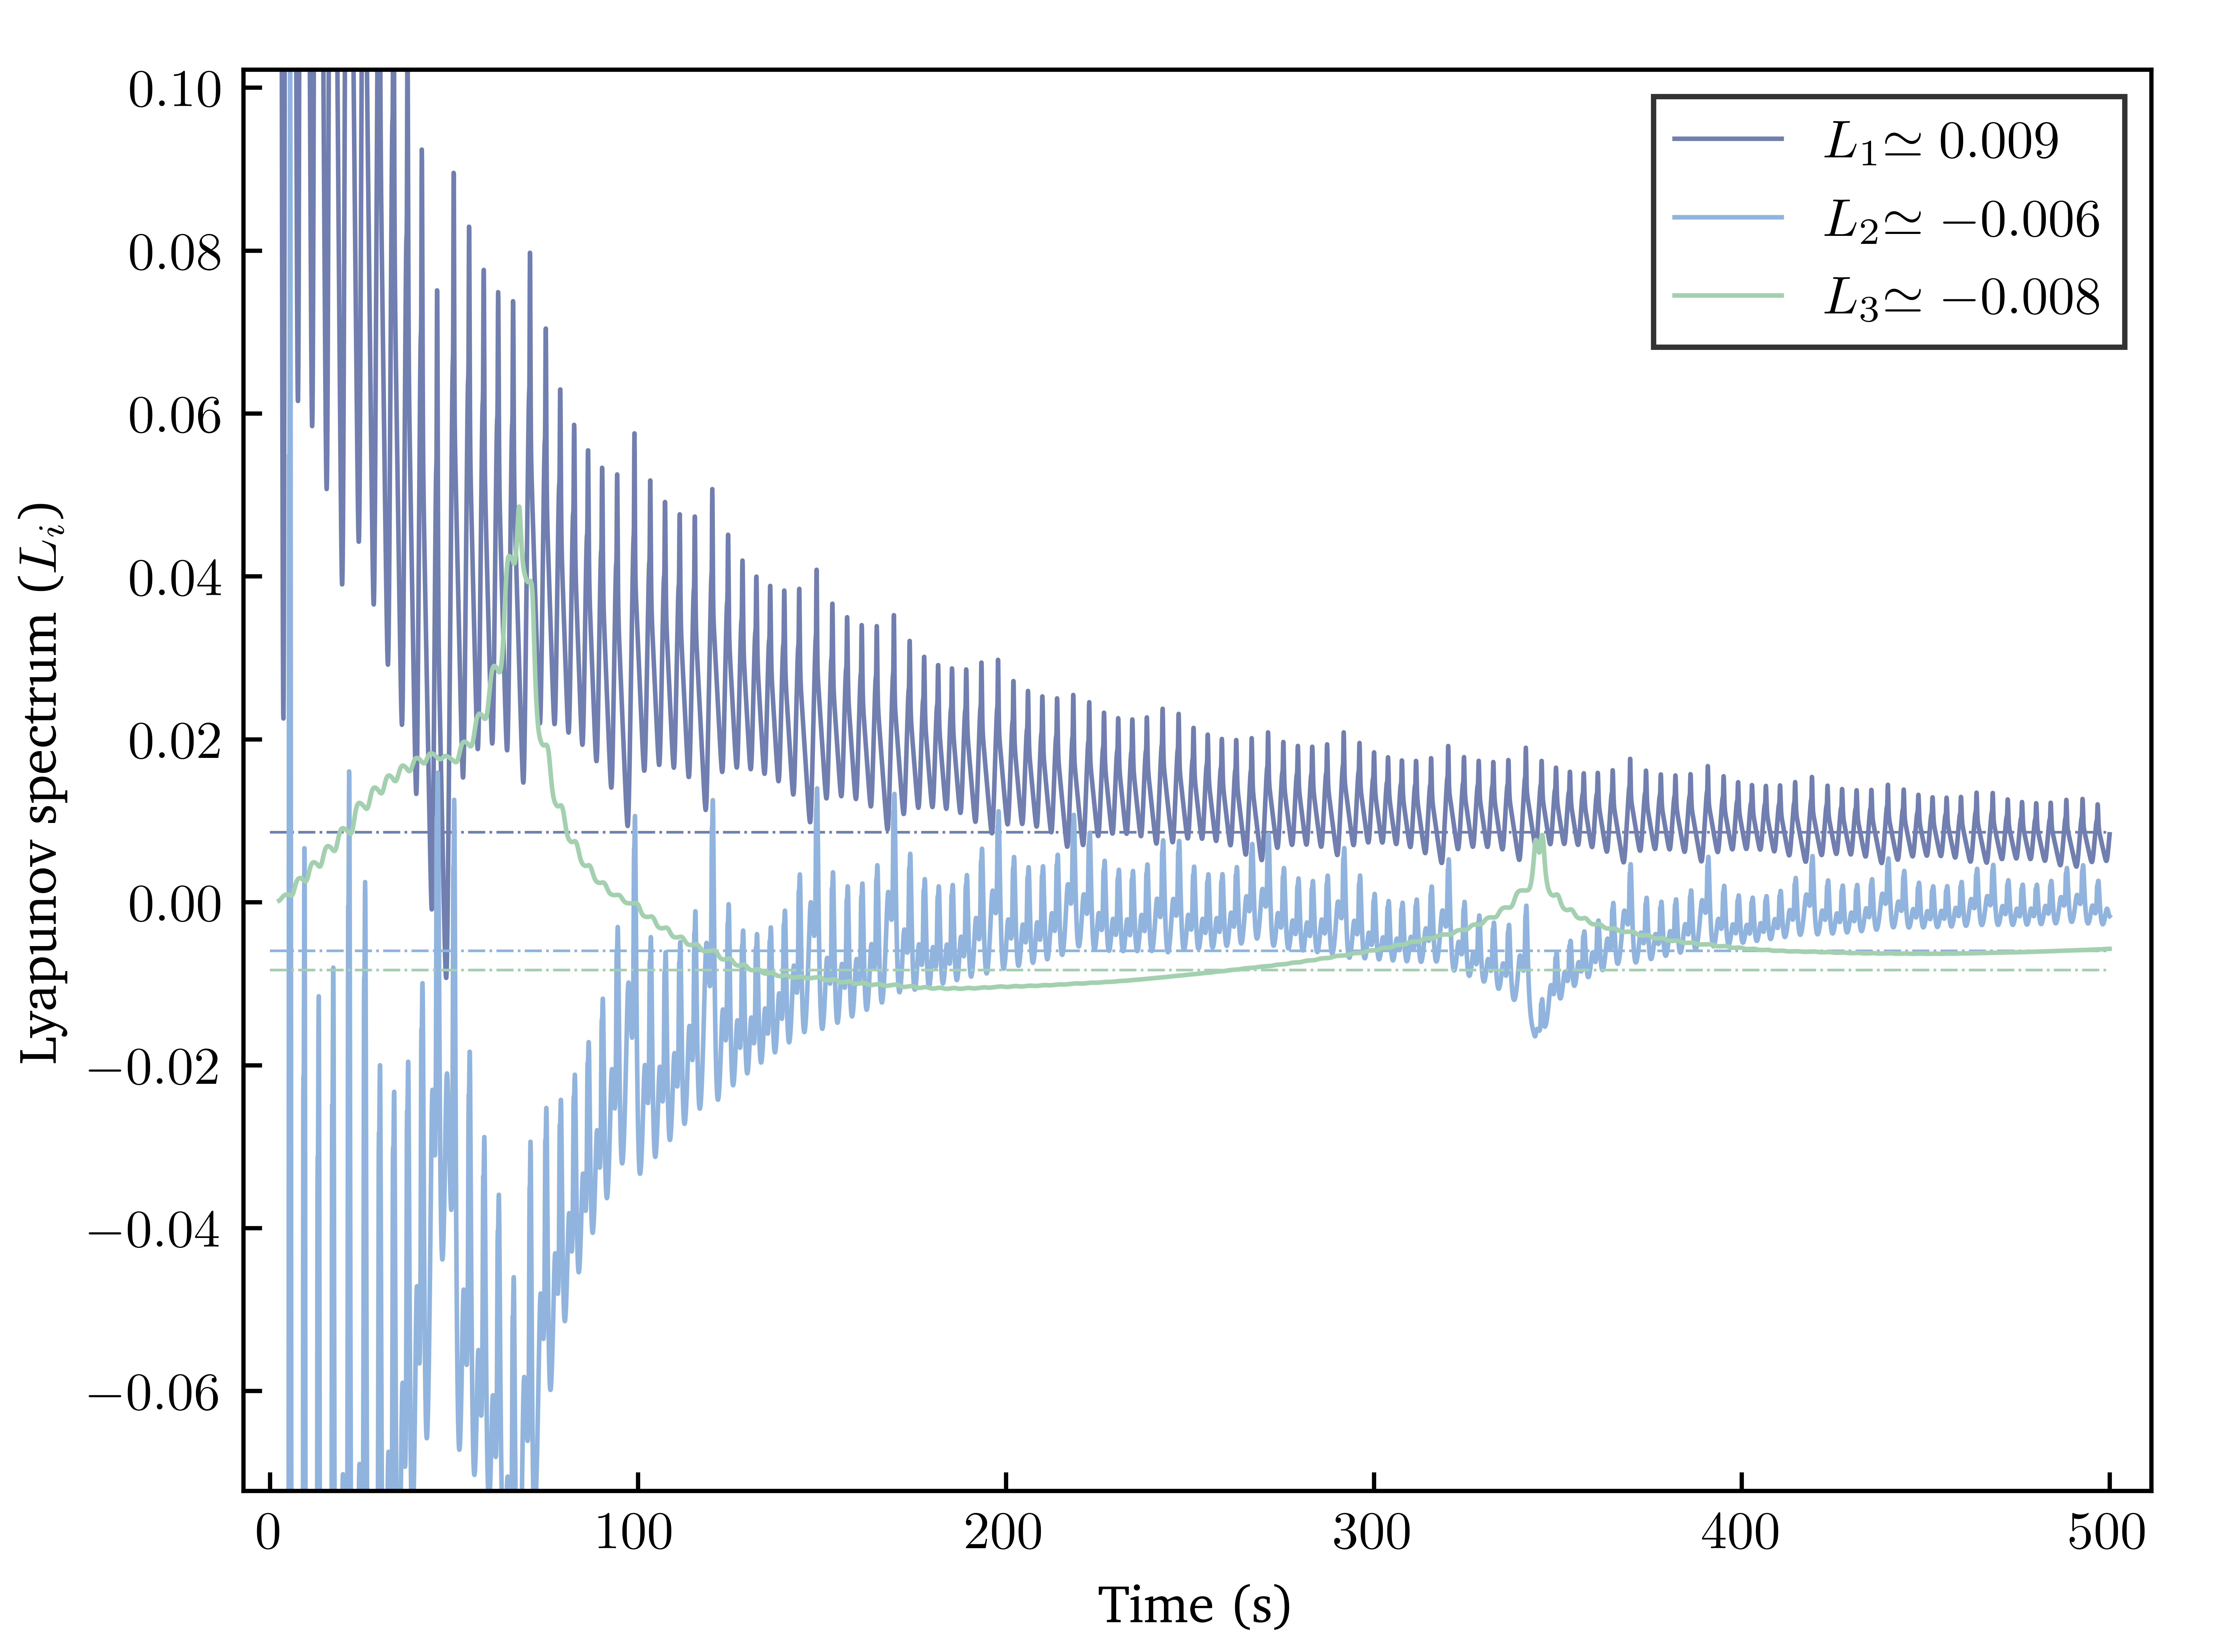
\includegraphics[scale=0.4]{figures/lyapunovs/lyap_bouali_zoom.png}
    \end{columns}
\end{frame}
